%%%%%%%%%%%%%%%%%%%%%%%%
%% Sample use of the infthesis class to prepare a thesis. This can be used as 
%% a template to produce your own thesis.
%%
%% The title, abstract and so on are taken from Martin Reddy's csthesis class
%% documentation.
%%
%% MEF, October 2002
%%%%%%%%%%%%%%%%%%%%%%%%

%%%%
%% Load the class. Put any options that you want here (see the documentation
%% for the list of options). The following are samples for each type of
%% thesis:
%%
%% Note: you can also specify any of the following options:
%%  logo: put a University of Edinburgh logo onto the title page
%%  frontabs: put the abstract onto the title page
%%  deptreport: produce a title page that fits into a Computer Science
%%      departmental cover [not sure if this actually works]
%%  singlespacing, fullspacing, doublespacing: choose line spacing
%%  oneside, twoside: specify a one-sided or two-sided thesis
%%  10pt, 11pt, 12pt: choose a font size
%%  centrechapter, leftchapter, rightchapter: alignment of chapter headings
%%  sansheadings, normalheadings: headings and captions in sans-serif
%%      (default) or in the same font as the rest of the thesis
%%  [no]listsintoc: put list of figures/tables in table of contents (default:
%%      not)
%%  romanprepages, plainprepages: number the preliminary pages with Roman
%%      numerals (default) or consecutively with the rest of the thesis
%%  parskip: don't indent paragraphs, put a blank line between instead
%%  abbrevs: define a list of useful abbreviations (see documentation)
%%  draft: produce a single-spaced, double-sided thesis with narrow margins
%%
%% For a PhD thesis -- you must also specify a research institute:
%\documentclass[msc,ai,twoside]{infthesis}

%% For an MPhil thesis -- also needs an institute
% \documentclass[mphil,ianc]{infthesis}

%% MSc by Research, which also needs an institute
% \documentclass[mscres,irr]{infthesis}

%% Taught MSc -- specify a particular degree instead. If none is specified,
%% "MSc in Informatics" is used.
 \documentclass[msc,ai,logo]{infthesis}
% \documentclass[msc]{infthesis}  % for the MSc in Informatics

%% Master of Informatics (5 year degree)
% \documentclass[minf]{infthesis}

%% Undergraduate project -- specify the degree course and project type
%% separately
% \documentclass[bsc]{infthesis}
% \course{Artificial Intelligence and Psychology}
% \project{Fourth Year Project Report}

%% Put any \usepackage commands you want to use right here; the following is 
%% an example:
\usepackage[round]{natbib}
\usepackage{draftwatermark}
\usepackage{hyperref}
\usepackage{float}
\usepackage[font=small,format=hang]{caption}
\usepackage{amsmath}
\usepackage{caption}
\usepackage[font=footnotesize]{subcaption}
\usepackage{slashbox}
\usepackage{graphicx}
\usepackage{epstopdf}
%% Information about the title, etc.
\title{Effect of Internal Models on Homeokinetic Controled  Autonomous Robots}
\author{Athanasios Polydoros}

%% If the year of submission is not the current year, uncomment this line and 
%% specify it here:
% \submityear{1785}

%% Optionally, specify the graduation month and year:
% \graduationdate{February 1786}

%% Specify the abstract here.
\abstract{%
   
}

%% Now we start with the actual document.
\begin{document}

%% First, the preliminary pages
\begin{preliminary}

%% This creates the title page
\maketitle

%% Acknowledgements
\begin{acknowledgements}

\end{acknowledgements}

%% Next we need to have the declaration.
\standarddeclaration

%% Finally, a dedication (this is optional -- uncomment the following line if
%% you want one).
 %\dedication{To my parents.}

%% Create the table of contents
\tableofcontents

%% If you want a list of figures or tables, uncomment the appropriate line(s)
%\listoffigures
%\listoftables

\end{preliminary}

%%%%%%%%
%% Include your chapter files here. See the sample chapter file for the basic
%% format.
\chapter{Introduction}
\label{ch:In}
The need for robots that can be used in real world drives researchers towards the development of intelligent and autonomous machines. Such machines should be capable to operate in complex environments that depend to many factors, thus the derivation of control rules that would achieve a desired result is challenging. The more widely used approaches belong to the class of evolutionary techniques \citep{nolfi2000evolutionary} but they have serious drawbacks.

 In the introductory chapter, will be presented, the attributes that robots should have in order to be characterized as intelligent and autonomous. Furthermore, will be mentioned, the main reasons that make the evolutionary strategies insufficient for real world applications and how their drawbacks can be overcome by adopting an approach inspired by the process of self-organization.Also, the definition of an internal model, will be presented, its significance at self-organized control and the research made in this field. Finally, will be mentioned, the motivation and the hypothesis of this thesis.
\section{Intelligent Robotics}
Nowadays robots are used in a wide range of applications. Companies that are operating on the fields of automation, space, defence are using robots for accomplishing tasks that are dangerous or hard for people, examples of such tasks are the assembly of heavy machine parts, underwater inspection of oil and gas pipes, diffusion of hazardous explosive devices, space exploration etc.

Those tasks are complex and taking place in extreme dynamically changing environment. This fact arises the need of robots that could cope with environmental changes, be easily adapted in different environments, perform slightly different tasks each time and operate without human intervention. This functionality can be achieved by developing intelligent autonomous robots. 

In robotics, the notion of intelligence can be interpreted as the ability of a robot to perform tasks that cannot be preprogrammed due to the uncertainty for the world state, thus an intelligent robot should be capable to improve its performance based on its experience and also has the ability of planning low-level actions for achieving a goal without being explicitly programmed. Finally, intelligent robots can adapt to environmental changes.

Autonomy is also an important feature of robots. An autonomous robot is not directly controlled by a human operator, and is not attached to an external power supply or an external processing unit. Among the most interesting principals are the self-regulation, self-organization and self-governing. Self-regulated robots can maintain a desired functionality despite the disturbances from their environment. Self-organization makes the robot capable to generate its own ability to perform actions and self-governing corresponds to the creation of own goals. Thus, autonomous robots are able to choose and change their behaviour by their own. 

Those principals are part of evolutionary strategies for robot control \citep{nolfi2000evolutionary} the common characteristic of evolutionary strategies is that they are biologically inspired thus the robots are developed based on a process that imitates the physical evolution. An initial population is initialized, the best individuals of this population are selected according to a performance criterion (fitness function), from those individuals the next generation is formed through evolutionary processes such as crossover and mutation. The next generation is also evaluated and the best individual are selected. The process terminates when the performance criterion is met.

The serious drawbacks of the evolutionary strategies are that they are time consuming and computationally demanding tasks \citep{Nolfi200231} since the performance of every single member of a population should be evaluated according to an evaluation criterion. Furthermore, the selection of this criterion is difficult because of the need to encode the possible states of the environment and also the desired low-level goals in a criterion, which could be impossible for a real, complex environment and task. Finally, at the application of evolutionary algorithm should be considered the limitations that are arising from the architecture of the robots and from the environment, such limitations have to be introduced as mathematical formulas, which could be a very complex task.Thus, modifications of the fitness function are required in case of changing environment or using a robot with different architecture.     

\section{Self-organization}
\label{s:SO}
A control scheme based on the principle of self-organization, deals with the described drawbacks of evolutionary strategies. According  to \cite{Haken:2008} self-organization is defined as:\textit{" The spontaneous often seemingly purposeful formation of spatial, temporal, spatiotemporal structures or functions in systems composed of few or many components"}. Thus, in a system which is initially disordered, through the self-organization process, arises some form of order or coordination between the agents that consist the system. This process is not triggered and does not depend on a single agent. 

A crucial characteristic of self-organization is that there is not a central control of the process, on the contrary the control is distributed in the entire system, which corresponds to a decentralized control strategy. Thus all the agents of a self-organized system contribute to the organization despite that they only interact locally. According to \cite  {Bonabeau:1999} [p.~9-11]  the self-organized systems exhibit three basic properties.First,is the existence of dynamical non-linearity, so a stimuli (input from the environment) results to a non-static output which, also, is not proportional to the input. Second, there is a balance between exploration and exploitation, the agents of the system do not only exploit their state  but they also exploring other potential states that could result to     a better state of the entire system. Finally, a large number of interactions between the agents occurs.     

The phenomenon of self-organization takes place in many systems such as physical, chemical and biological systems. An example of self-organization in biology is the formation of a swarm of animals like birds, fishes, wolves. Figure \ref{fig:swarm} illustrates the formation of a swarm of birds, this formation is a result of self-organization. 

\begin{figure}[h]
\includegraphics[scale=0.25]{swarm.jpg}
\centering
\caption{Birds' swarm as result of self-organization}
\label{fig:swarm}
\end{figure}
\include{Introduction}

This formation is not controlled by a single individual but occurs based on negatives and positives feedbacks from the agents. Those feedbacks depend on a high-level goal. At this particular example the formation is a result of two opposing goals. The need of birds for immigration and dealing with threats such as predators. Thus if they attempt to fly away from the swarm there is a high risk because they are more vulnerable to predators and the coordination arises because all the individual want to immigrate. In many examples the occurrence of self-organization is the result of two opposing forces. The swarm will exhibit a variety of patterns according to the environmental stimulus such as the wind, the existence of a specific threat, need for food e.t.c. This results to the emergence of new capabilities of the system.

Based on the definition and the provided example of self-organization, could be concluded that using this principal in a single robot, considering as system the robot and its environment as agents the robot's motors and sensors that would sense the environment, should occur a coordination of motors in order to achieve a defined high-level goal. The robot does not know \textit{a priori} how to achieve this goal, so it has to generate sensorimotor coordination, through this coordination, a wide range of behaviours can occur. 

Thus, in contrast with evolutionary strategies the computational complexity can be kept low because in self-organization process the change of an agent's state does not affect the whole system and also the limitations that arising from the configuration of the robot and from the environment are not introduced with explicitly because a self-organized controller produce motor commands that fit to the embodiment. The concept of embodiment is crucial, the robot's brain, body and environment have to be treated as unity \citep{Brooks91} because the self-organization process relies on a continuous interaction between the agents and the environment.

Thus, the control scheme of the robot should include two characteristics because of the continuous interaction with the environment and the need for feedback from the agents. Namely a closed loop, through which the controller receives the effect of the motor commands   and an internal model, which encodes the belief of the agents about the environment.

\section{Internal model}   

The use of internal model in robots is biologically inspired and exist in a large number of biological organisms, it is believed that the central neural system performs transformations between the actions and the sensory states. According to \cite{Kawato1999718} \textit{"Internal models are neural mechanisms that can mimic the input/output characteristics, or their inverses, of the motor apparatus"} thus internal model represents the belief of an organism about its environment.There are numerous researches and experiments that prove the existence of internal model in humans \citep{Wolpert29091995,Flanagan97therole, Thoroughman2000}.

 For instance, in \cite{Thoroughman2000}  the existence of an internal model was proved using a simple experiment in which subjects where ask to perform reaching movements at a plane towards a desired plane holding a robotic manipulandum, which produced viscous forces. After a number of trials where the viscous force is applied the subjects reduced the error between desired and actual position, when a catch trial occurs (viscous force is not applied) the error becomes large and has opposite direction compared to the field trials, which denotes the existence of internal model.
 
 Thus, the use of an internal model in the control scheme of a robot could be interpreted as adding consciousness in the robot. An interesting use of internal models is presented in \cite{Bongard2006} 
where, the authors, motivated by the ability of animals to be functional after the occurrence of an injury, they developed an algorithm that applied in a four-legged starfish robot. It uses relationships between actions and sensations in order to infer its configuration and then it uses a self-model for achieving a desired locomotion. The self-model is based on multiple competitive internal models, thus it is capable to adjust its self-model when a leg-part is removed and create an alternative gait for moving. 
 
A recent survey on internal models that are used for robot control was made by \cite{Nguyen-Tuong2011}. The type of used internal models depends on the prediction problem, so there are three main types of internal models the forward, the inverse and the mixed problem.
Figure \ref{fig:im} illustrates a general example of a plants' control scheme using a forward internal model as a representation of the plant. Forward models perform a mapping from the control signal to the predicted state of the plant, thus it is a prediction of the state of the process if the control signal emitted by the controller will applied at the plant. The inverse model performs the opposing function, given the state of the plant it reconstructs the control signal that was applied to the plant and had as result the observed state, thus they do not represent a cause-effect relationship but an effect-cause. A problem of those models is that the effect-cause relationship is, in some cases, ill-defined. This happens when the output space is not convex \citep{COGS:COGS236}. A mixed model is a combination of a forward and an inverse model and were introduced in order to overcome the problems that arising from the use of inverse models. 
 
 \begin{figure}
\includegraphics[scale=0.6]{im.png}
\centering
\caption{Control scheme with forward internal model}
\label{fig:im}
\end{figure}

The forward models are generally used in robots in order to achieve fast movements with high compliance and adaptation to changes. This is achieved by using the closed loop setup. The error between the true and the predicted state of the plant is fed-back to the controller and is taken into account for the generation of the next motor command.Thus, the controller smoothly corrects the state of the plant and makes the control system capable to cope with unexpected changes of the plant state.

An interesting attribute of internal models is the efference copy.In biology, it is believed that the signals emitted from the central neural system are copied locally and makes the organisms capable to distinguish between the sensory inputs that were a result of the organism action and those that were a result of environmental stimuli. The effect of the efference copy at the internal models' predictability in robotics was investigated by \cite{Schroder} and \cite{Manoonpong}    

\section{Background}
In this section will be presented the previous work made on the research field of the self-organized control on autonomous robotics. The introduce of the self-organization principle in machines was made by \cite{Neumann} where a machine that has knowledge about its own configuration can assemble itself. This work is based on theoretical concepts and is not concerned about the practical implementation but it was the basis for research in the field of self-organization of physical systems \citep[p~.38]{murata2012self}. 

The research is mainly focused on applying the self-organization principle in systems that consist of several robots (multi-robots systems and swarm robotics). An influencing research on this field was made by \cite{Reynolds}, who proved that the emergence of a flocking behaviour can be achieved by using simple rules that describe the local interactions between the agents. Also the patterns of the flock change according to attributes such as the noise  of the system, the density of the flock and the parameters of the local interactions, also the agents of the systems tend to keep a distance between each other while they perform complex tasks such as obstacle avoidance. Thus, a very complex high-dimensional system can be controlled through the adaptation of a small number of parameters. One drawback can be considered that those findings are result of simulations, the difficulty of applying those principal in real robots rise significantly in real world applications due to the environmental complexity and the robots' configuration.

A research about the emergence of self-organization in a group of physical robots was made by \cite{Trianni} the study was focused on the generation of self-organized behaviour for a group of robots. Their movement is coordinated through communication strategies, a variety of such strategies were tested and the findings denote that evolutionary controllers produce a robust self-organized system. Similar researches on swarm robotics were made by \cite{Svennebring} and \cite{Nuyan}. The same characteristic at the application of self-organization on robot swarm is that they investigate the behaviour of a group of robots and not of an individual robot which would result the generation of capabilities, instead the individuals are controlled through a decentralized control technique.       

Different robot behaviours can emerge by using the homeokinetic controller which was introduced by \cite{dersteinpas99}. Based on the fact that the artificial evolution of an individual can be significantly fast if the individual can learn fast its embodiment, the authors used the principle of homeokinesis which, despite the fact that is completely unspecific gives rise to specific behaviours. Also, the importance of an adaptive internal model is underlined. The general goal of this principle is to keep the agent in a kinetic state which can be predicted by the internal model, thus this principle can be considered as the opposite of homeostasis, which is the ability of a system to maintain a stable state. Despite that, in this article, the proposed method is tested on linear and non-linear control tasks only by simulations there is a number of subsequent researches that this principal was tasted in both simulated and real robots.

Particularly in \cite{der01} the homeokinetic controller was tested in a real Khepera robot. The aim of the research was to investigate the emergence of situated behaviours on a robot controlled by the principal of homekinesis. A situated behaviour is defined as the behaviour of an agent who controls its actions by using the maximum sensory information. The experimental results proved the assumption that different behaviours can emerge from the homeokinetic principle using the same internal model and learning parameters, namely the robot was able to avoid obstacle, navigate through corridors and complex mazes and to follow walls.

\cite{derhesselieb04} examined the ability of the homeokinetic controller for sensory integration, to use the sensor inputs that origin from both the agents' body and environmental stimuli in order to use its body effectively within the environment. This is achieved by using simple learning rules for the controller that result to an automatic integration of the sensors after they emit a signal to the controller. The interesting findings of this research was that the sensory integration make the robot capable "survive" in a simple world also the system is not affected by problems that occur when the sensor properties change rapidly. Also the robot adopts an explorative behaviour which, however depends from the environment. 

It is clear that the principle of homeokinesis does not specify a goal for the agent. This issue is solved by guiding the behaviours that emerge from the self-organization process towards a desired goal \citep{martius:guid} according to this approach reinforcement signals are used to shape the behaviour of the robot (negative signals for punishment and positive for reinforcement). The experiments applied this approach for achieving desired spin and speed in different robots. Also the effect of different signal strategies were examined \citep{martiusherrmann}. Finally, a summary of the research on goal-free and guided self-organization was made by \cite{DerMartius11}

\section{Motivation}   
The previous sections illustrated the significance of self-organization to the evolution of intelligent robots. The main characteristic that makes this research field interesting is that machines can produce their own capabilities without being given a specific goal, such capabilities could be too complex to be preprogrammed with explicitly. Through the self-organization process we can mimic the sensorimotor coordination that occurs in real life, this results to the emergence of behaviours that depend on the body and the stimuli of the environment. For example, humans are not taught with explicitly how to walk and also they are not given a direct goal to achieve it. The walking behaviour is result of exploiting the intrinsic capabilities and exploring the environmental stimuli.

The homeokinetic principle that is used in this thesis is based on the self-organization process that takes place in nature. The research that has been made on its application on robotics exhibits interesting results about the behaviours that emerge since relatively complex behaviours are developed despite the simple environment and internal model that were used. Furthermore, since this principle is goalless, it could be safe to say that robots are acting based on an intrinsic motivation. 

Also, the research does not investigates the impact of different types of internal models on the generated robots' behaviours. As it will be presented in the next chapter, the homeokinetic controller depends on both the inner dynamics of the internal model and its prediction accuracy. Thus, both the complexity and the predictability of the model should have an impact on the behaviours.

Finally, the dependence between the emergence of explorative behaviour and the internal model, will be examined  since robots that have an explorative behaviour can be used in many real world applications.

\section{Hypothesis}   
\begin{itemize}
\item The complexity of the environment affects the complexity of generated behaviours.
\end{itemize}
Based on the fact that self-organized processes which occur in nature are heavily depended on the environment, it is logical to hypothesize that complex environments drive the robot to generate more complex behaviours than the simple environments. 
\begin{itemize}
\item The quality of the model affects the generated behaviours
\end{itemize}
As indicators of model's quality will be used, the mean squared error between the actual and the predicted state and the area of the environment that was covered by the robot. Through this will be examined if better predictors result to inactivity because the robot falls into an uninteresting regime.
\begin{itemize}
\item There is a dependence between model and environment complexity
\end{itemize}
Since more complex predictors perform better at the approximation of complex functions compared to simple predictors, it would be interesting to investigate if complex internal model perform better in complex environments and as result are driving the robot towards an exploratory behaviour.
\begin{itemize}
\item Complex models result to complex behaviour 
\end{itemize}
Based on this hypothesis the models that have complex inner relationships can adapt faster to a change of the target function that they predict, contrary to simple models that need much time to adapt in changes. This could result in complex behaviour because the fringe states that may occur would be learned faster from the agent. Despite that the term of behavioural complexity is fuzzy, a method has been proposed by \cite{ay08}. N. Ay and colleagues, measured complexity in terms of the predictive information in sensor space. 

\section*{Thesis outline}
In Chapter ~\ref{ch::hom} will be presented the structure of closed loop control scheme and the main reasons that make this scheme important. Also, will be explained the sensorimotor loop and its significance in self-organized control. Finally, the derivation of the homeokinetic principal will be introduced.    

Chapter \ref{ch::int} includes a presentation of the internal models that will be used, the basic reason for selecting those, their possible advantages and disadvantages, the derivation of the learning rules and references to research areas that were successfully applied.  
 
The evaluation procedure that will be used for testing the hypothesis will be presented in Chapter \ref{ch::ev}. Also, will be mentioned, the setup of the  experiments, including the different environments and description of the used robot. Finally, the results of the evaluation process will be illustrated.

In Chapter \ref{ch::ev} is contained the outcome of the results, a discussion about how the findings validate the hypothesis and possible drawbacks of this approach. Finally, will presented directions for future work on this research field.   
\include{Introduction}   

\chapter{The Homeokinetic control scheme }
\label{ch::hom}
The homeokenetic controller is applied on a closed loop scheme. The advantages of the closed loop control, such as the feedback and the representation as a dynamical system enables the derivation of simple learning rules for the controller. Based on those learning rules the robot can exhibit a variety of behaviours that fit its body and environment (embodiment). In this approach there is not any external teacher who will favour a specific kind of behaviour, thus there is not a desired goal. There are two intrinsic high-level goals that have to be achieved. Namely, the robot should be able to active and be able to predict the results of its actions in the environment.  

\section{Open and closed loop control}
Figure \ref{fig:openloop} illustrates a general open loop control system. The reference or desired value is fed to the controller, in most control systems there is a process unit which converts the input into a form that can be used from the controller, the controller emits a noise contaminated command signal which is applied to the controlled plant and produces an output. 

\begin{figure}[h]
\includegraphics[scale=0.5]{openloop.jpg}
\centering
\caption{Open loop control scheme}
\label{fig:openloop}
\end{figure}

The main characteristic of this control scheme is that it cannot take care of any disturbances that adds to the emitted command signal from the controller and any noise that could affect the output signal. Hence, open loop systems are unable to detect and correct any disturbances that occur and they are only commanded by the input. As result open loop control schemes are not only sensitive to noise but also are unable to detect and correct the disturbances that occur.
Despite those drawbacks they are applied in simple processes where the output is controlled by external factors because of their simplicity and low cost. 

An example of open loop control is presented by \cite  {DerMartius11} [p.~39]. This experiment consists of a barrel that is moved by two internal heavy weights that slide on two perpendicular axis. The weights are controlled by a linear motor, thus the by sifting the weights the barrel changes its center of gravity, the weights' movement result to the system's movement. The experiment starts by using a periodic control signal which changes the weights with a phase sift of $ \pi/2 $ then the frequency is doubled over the time in order to achieve a higher rolling speed. This results to a sacadic motion of the barrel and makes clear that the open loop control is insufficient for generating a smooth fast motion of the barrel.   

The drawbacks of the open loop controlled systems can be overcome in closed loop systems. A general architecture of that kind of systems is illustrated in figure \ref{fig:closloop}. The reference signal, desired plant state, is often translated into a form that is interpretable from the controller. For instance if the controller uses electrical signals to operate the motors of a robotic arm and the output of the system is the pose of the arm, then the pose have to be converted to electrical signals. 
\begin{figure}[h]
\includegraphics[scale=0.6]{closedlloop.jpg}
\centering
\caption{Closed loop control scheme}
\label{fig:closloop}
\end{figure}

After the translation of the output the feedback signal is subtracted from the reference creating the actuating signal or error. This actuating signal is fed to the controller which generates the necessary motor commands in order to regulate the plant towards the desired output. Thus the closed loop control systems can deal with disturbances by measuring the output of the plant, feeding back the output measurements through a feedback plant and comparing the output with the desired input. If the desired input is different from the output the controller uses that difference in order to adjust the output, in case that there is no difference between the desired and the current state there is not an actuating signal and the controller does not drive the plant because it is already operates in the desired state.

It is obvious that closed loop systems are more accurate than the open loop systems because they have a limited sensitivity to noise, disturbances and external (environmental changes). On the contrary those systems are more complicated since they need an output sensor and a converter for translating the output signal as described above. Thus, it is also more expensive.

Despite the disadvantages, for taking into account the interaction between the agent and the environment,which is crucial for developing self-organized machines, the use of a closed loop control scheme seems to obligatory.  
Thus, in this way, the agent is able to adjust its behaviour based on the environmental stimuli. But also, as it is already mentioned in the previous chapter, there is not a specific desired output that is set to the agent extrinsically, instead the goals are result of an intrinsic process. Thus, in the homeokinetic control scheme is used the biologically inspired concept of the sensorimotor loop.

\section{The sensorimotor loop}   

The concept of sensorimotor loop signifies the strong dependence between sensory input and motor output in a closed loop cycle. Its importance in biological agents is highlighted in a number of researches \citep{wiener,Ferezou,Nguyen} this inspired it application in robotics. The figure \ref{fig:sensorimotor} illustrates the process of a sensorimotor loop in humans.

The approach of homekinesis is based on applying  closed loop control in a sensorimotor loop, this makes possible an implementation of closed loop system without an externally defined reference value (desired output of the system). Thus, any change on the controller (motor commands) is driven by the state of the sensors, this fact makes the robot capable to act according to intrinsic parameters instead of acting based on an external goal and the result can be interpreted as emergence of self-organized behaviour. 

\begin{figure}[H]
\includegraphics[scale=0.7]{sensorimotor.jpg}
\centering
\caption{The sensorimotor loop in humans \citep{Wolpert2}}
\label{fig:sensorimotor}
\end{figure}
 
An implementation of the sensorimotor loop is presented in figure \ref{fig:snsRobot} in a simple case with one input and one output. At every time step $ t=0,1,2,3,... $ the controller $ K $ receives the sensor values $ x_{t}$ and generated motor commands $y_{t} $ the motor commands are applied to the robot $R $ which interacts with the environment and, by this way, the new sensor values $x_{t+1}$ are generated and are fed to the controller as input at time step $t+1$. Thus $x_{t} \in I $ and $y_{t} \in O$ where $I$ and $O$ are the sensors' and motors' space respectively.

\begin{figure}[H]
\includegraphics[scale=0.35]{sns.jpg}
\centering
\caption{Application of sensorimotor loop in robotics}
\label{fig:snsRobot}
\end{figure}

Thus, the controller in the sensorimotor loop performs a mapping $K: I \rightarrow O$ according to the following equation
 \begin{equation}
 \label{eq::ConGen}
y_{t}=K(x_{t};C,h)
\end{equation}
where $x_{t}$ is the current sensory inputs and $C,h$ are adjustable parameters of the controller. The controller of the homeokinetic control scheme represents a single neuron, thus equation \ref{eq::ConGen} can be rewritten as:
\begin{equation}
\label{eq:controller}
y_{t}=K(x_{t};C,h)=\tanh(Cx_{t}+h)
\end{equation}  

So the parameters $C$ and $h$ can be interpreted as the 
the synaptic weights and the bias term respectively. The function $\tanh$ is the hyperbolic tangent which belongs to the class of sigmoid functions and is used for keeping the motor commands within the desired interval $y_{t} \in [-1,1] $.

Since the motor commands are applied to the robot which is interacting with the environment the sensor's values are changing according to the configuration of the robot. Thus the transformation of the motor commands $y_{t}$ to the new sensor values $x_{t+1}$ can be represented by a function $W(y_{t})$ which performs a mapping from motor's space to sensor's space $W: O \rightarrow I$
and the sensor value is defined as 
\begin{equation}
\label{eq:world}
x_{t+1}=W(y_{t})+ \xi_{t}
\end{equation}

Where $\xi_{t}$ are disturbances such as noise. The function $W$ represents the world, and assuming that the processes taking place in the world are unknown we need to approximate them using an internal model which is implemented by the function $M(x_{t},y_{t};w)$. Thus $M(x_{t},y_{t};w)$ performs, also, a mapping from the motor commands to the sensor's space. By adjusting the model's parameters $w$ based on the prediction error, the difference between the predicted sensor values and the the true sensor values (output of function $W$), we can obtain a better approximation of the world. The significance of the internal model on the homeokinetic control principle will presented with explicitly in the next sections of this chapter.

Assuming a simplified world defined as 
\begin{equation}
•W(y_{t})=a y_{t}
\end{equation}

 The equation \ref{eq:world} can be written as 
 
 \begin{equation}
 \label{eq:wor}
•x_{t+1}=a y_{t}+ \xi_{t}
\end{equation}
 
Where $a$ is an unknown constant. From the equations \ref{eq:wor} and \ref{eq:controller} is derived the complete equation of the control system.
\begin{equation}
\label{eq:comp}
•x_{t+1}=\psi(x_t) = a \tanh(Cx_{t}+h)+ \xi_{t}
\end{equation}

Equation \ref{eq:comp} can be interpreted as a non-linear neuron model with self-connection, the neuron is activated from the stimuli that are generated from itself. The dynamics of such types of neurons were the research topic of numerous researchers \citep{Renals,Pasemann1993}. Thus the complete equation of the system can be written in terms of membrane potential of the neuron.

\begin{equation}
z_{t+1}=r \tanh(z_{t})+h
\label{eq:potential}
\end{equation}

Where $z_{t}=Cx_{t}+h$ and $r=Ca$. The study of the dynamics of the controller in terms of the membrane potential is crucial for anticipating the way that the controller changes the generated motor commands.

\section{Sensorimotor loop dynamics}

Before the illustration of the homeokinetic controller's  dynamics, it is useful to present a general case of a controller's dynamics in order to anticipate how the movement policies can be represented as dynamical systems and the benefits of such representation. Given that there is a desired state of the system, the goal is the derivation of a differential equation that will have a stable attractor landscape the attractors can be modified through a learning process.

A differential equation can have fixed points, if $f(x)$ is differentiable and $x$ is a fixed point, then it is true that $f(x)=x$. Thus the fixed point do not change from the application of mapping $f$. The fixed points could be attractors, repellers or saddle points. Attractors are points towards which a variable evolves over time according to a dynamical system. Reppelers have exactly the opposite properties from the attractors and saddle points are also stationary points but they are not extrema (reppelers or attractors). Thus a dynamical system changes states according to the positions of attractors and reppelers and by representing a control scheme as dynamical system we can obtain a better understanding about the rules that define its operation.

For interpreting the properties of the membrane potential as a dynamical system, we should examine the fixed points of equation \ref{eq:potential} The fixed points of the membrane potential can be found either graphically or analytically using the series expansion theorem \citep{martius:diss10}. Figure \ref{fig:biffuc} illustrates the change of the fixed points depending on the value of the feedback weight $r$ and for $h=0$. If the value of $r$ is less than $1$ then there is a single fixed point at $z=0$, for values of $r$ greater than $1$ the previous fixed point becomes unstable and new stable points appear. The interesting fact is that the fixed points which appear if $r>1$ has opposing signs. 

\begin{figure}[H]
\includegraphics[scale=0.5]{biff.jpg}
\centering
\caption{Fixed points of membrane potential as a function of $r$ \citep{hesse09:diss} }
\label{fig:biffuc}
\end{figure}

Based on this fact it is clear that a bifurcation appears. According to \cite{Guckenheimer:2007} the bifurcation of a dynamical system, is defined as: \textit{"The qualitative change in system's dynamics produced by varying parameters." }. Thus at the systems with this property a small change of a parameter results to a sudden change in its behaviour. Furthermore it was proved that the bifurcation created from the derivative of membrane potential function is a special case of bifurcation, namely a cusp bifurcation \citep[p.~37]{martius:diss10}

This property, in the example of one-dimensional controller, will result to a robot that would not move when $r<1$ and it will move forward or backward if $r>1$. The direction that it will take is not a result of an intrinsic choice but is the result of the symmetry breaking phenomenon which occurs in bifurcations and the system follows a branch of bifurcation according to small fluctuations that occur in the system (noise).Thus, in order to generate motion is crucial to maintain the value of $r$ above the critical point and since $r=Ca$ this is achieved by changing the parameter $C$ because $a$ is constant.   

So far the impact of the bias $h$ is not examined since we assumed that $h=0$, but it also has impact on the occurrence of fixed points. A detailed investigation on the effects of the bias term is presented by \cite{hesse09:diss}. It was proved that, assuming a critical value of the bias $h_{c}$ where a symmetry breaking occurs, and if it is true that $h>h_{c} \vee h<-h_{c} $ three fixed points are created. Figure \ref{fig:biffuccat} illustrates the case $ h<-h_{c} $ if 
$h>h_{c}$ the only change is that the fixed points change sign. From this illustration can be concluded that a merge of two branches occurs resulting to a catastrophic bifurcation. 

\begin{figure}[H]
\includegraphics[scale=0.47]{biffcat.jpg}
\centering
\caption{Fixed points of membrane potential as a function of $r$ and $h<0$ \citep{hesse09:diss} }
\label{fig:biffuccat}
\end{figure}

There are three fixed points, two stable (continuous lines) and one unstable (dashed line) when the value of bias slowly changes (increases or decreases) the state of the system can be found in one of the two stable fixed points and remains at this stable point until its fixed point disappears due to the change of the bias. Then it jumps to the fixed point that has the opposite sign \citep{martius:diss10}.Thus, the parameter $C$ controls the two possible states of the system,a change of this parameter produces two new possible states. The parameter $h$ controls the transition between those two states. Therefore, is suitable to maintain the parameter $r$ above the bifurcation point and change the bias in order to achieve a transition between the two states/    

The analysis of the sensorimotor loop dynamics shows that, using a closed loop system with a controller which can be realized as a single neuron with self feedback weight, fixed points are found that can be adapted in order to achieve a self-organized behaviour based on the principle of homeokinesis. 
\label{dynamics}
\section{Principle of honeokinesis}
In the previous section \ref{dynamics} was illustrated that exploiting the dynamics of the sensorimotor loop, different states of the systems can be emerge. A small change of the parameter has as result a change of the system which is common phenomenon in the self-organized processes. In order to have a self-organized system we need to derive a method for adapting the parameters of the sensrimotor loop ($r,h$) that would have common characteristics with the rules that cause self-organization in systems.   

If the minimization of the prediction error is used (as illustrated in figure \ref{fig:snsRobot}) will result in a static behaviour because the system will prefer states that can be easily predicted from the model. Therefore the robot would not move because it could predict with bigger accuracy a stable state. Thus, we need a principal which will drive the system in changing its state resulting into an active and innovative robot. This issue is solved using a control scheme based on the principle of homeokinesis which could be characterised as a supervised learning algorithm but using a learning rule that is internal to the agent. The goal of this rule is to adapt the parameters $r$ and $h$ in order to generate a class of behaviours that will be explorative and fit the agents' embodiment.

 For achieving the described operation of the system \cite{derlieb02} proposed the Time Loop Error (TLE) as objective function used for the adaptation of parameters $r$ and $h$. This adaptation requires knowledge of the unknown hardware constant $a$ therefore an internal model is used in order to approximate this factor. The control scheme that applies the principal of hoemokinesis for robotic control is illustrated in figure \ref{fig:homeo}. This control scheme will be used in this thesis.

\begin{figure}[H]
\includegraphics[scale=0.75]{homeo.png}
\centering
\caption{Sketch of the homeokinetic control scheme }
\label{fig:homeo}
\end{figure}

The time loop error is derived by back-propagating the sensor values $x_{t+1}$ throw the internal model, this results to the derivation of predicted motor commands $\hat{y}_t$ which can be interpreted as an estimation of the actual motor commands, then the predicted motor commands are also propagated back through the controller and the reconstructed sensor value are derived.

The robot's intrinsic anticipation of the sensorimotor loop can be formulated as 
\begin{equation}
x_{t+1}=\psi(x_{t})+\xi_{t}
\end{equation}
 
Where  $\psi(x_{t}) = M(K(x_{t}))$ and $\xi_{t}$ the prediction error at time step $t$. As result, in each time step, the sensorimotor loop transforms the input $x_{t}$ to the  output $x_{t+1}$. The reconstruction of the input based on the observed output is equivalent to 
the calculation of an input shift $u$ such that 
\begin{equation}
x_{t+1}=\psi(x_{t})+\xi_{t}=\psi(x_{t}+ u_{t})
\label{eq:sift}
\end{equation}


Thus the parameter of the input shift can be realized as the change that should occur at the sensor input in order to compensate for the prediction error $\xi$ \citep[p.~42]{martius:diss10}. Assuming that the inverse of function $\xi$ exists, the reconstructed sensor values can be written as

\begin{equation}
\hat{x}_{t}=x_{t}+u_{t}=\psi^{-1}(x_{t+1})
\end{equation}  

Thus, a quantity $u$ that represents the input shift can be written as the difference between the true and the reconstructed sensor values. 

\begin{equation}
u_{t}=\hat{x}_{t}+x_{t}
\end{equation}  

The goal of the homekinetic control scheme is to minimize this value which can be calculated assuming that it is small and thus we can use a Taylor expansion, so the last part of equation \ref{eq:sift} is written as  
\begin{equation}
\psi(x_{t}+ u_{t})=\psi(x_{t})+L(x_{t})u_{t}
\label{eq:taylor}
\end{equation}

Where $L$ is the Jacobian of the sensorimotor loop and is defined as 
 
\[L = \frac{{\partial \psi ({x_t})}}{{\partial {x_t}}}\]

Thus the input shift can be derived using the equations \ref{eq:sift} and \ref{eq:taylor} as follows 

\begin{equation}
{u_t} = \frac{{{\xi _t}}}{{{L_t}}}
\end{equation}

Finally the time loop error is defined as 
\begin{equation}
TLE=\left|{u_t}\right|^2 = {\left| {\frac{{{\xi _t}}}{{{L_t}}}} \right|^2}
\label{eq:tle}
\end{equation}

Minimizing the time loop error can be realized as finding the best trade-off between the change of the sensor value and the prediction error. It consists of two parts, the prediction error and the Jacobian, for minimizing the time loop error we need to minimize the prediction error and maximize the Jacobian.
 The Jacobian can be interpreted as a measurement of the system's sensitivity because it represents the rate of the output's change with respect to the input, the maximization of the sensitivity drives the system to activity on the contrary the minimization of the prediction error drives the robot to "prefer" highly predictable states.
 
 It is clear that two opposing forces are acting to the system, the need for high sensitivity and the predictability. The two opposing forces that act to a system is common phenomenon in real life, for instance, at the example of the birds' swarm presented in section \ref{s:SO}, two opossing force are acting, the need for immigration and the threat from predators. If the birds do not want to immigrate then they remain hidden in their nests because of the predators, on the other hand, if there was not a threat then the birds will not formate a swarm.   
\label{sec:tle}
\section{Learning rule}

The learning rule of the controller involves the calculation of the gradient of the time loop error. For keeping the simplicity of the formulas, the derivation of the learning rule in one-dimensional case will be presented and a simple linear model will be defined as 
\begin{equation}
M(y)=ay+b
\label{eq:model}
\end{equation}

 Recalling the formulas that describe the system, denoting as $g(z)$ the activation function of the controller such that $g(z)=\tanh(z)$ and neglecting the time-step indicator $t$ it is true that 

\[K(x)=g(Cx+h)\]
\[\psi(x)=M(K(x))=a(g(cx+h))+b\]
\[L=\frac{{\partial \psi ({x_t})}}{{\partial {x_t}}}=acg'\]

Where $g'$ and $g''$ are the first and second order derivative of the sigmoid function $g(cx+h)$ Then, the gradient of the time loop error (equation \ref{eq:tle}) with respect to the parameter $C$ can be calculated as follows
\begin{equation}
\Delta C =  - \varepsilon \frac{{\partial {\rm E}}}{{\partial C}} =  - \varepsilon 2\frac{\xi }{L}\left( { - \frac{\xi }{{{L^2}}}\frac{{\partial L}}{{\partial C}} + \frac{1}{L}\frac{{\partial \xi }}{{\partial c}}} \right)
\label{eq:grad}
\end{equation}
Using in equation \ref{eq:grad} that 
 
 \[\frac{{\partial L}}{{\partial C}} = ag' + acg''x\]
 \[\frac{{\partial \xi }}{{\partial C}} = 0\]
 
 It can be simplified to the form 
 
 \[\Delta C = \varepsilon \frac{{{\xi ^2}}}{{{L^3}}}(ag' + acg''x)\]
 
 Which can be further simplified using a time-dependent learning rate ${\varepsilon _t} = \varepsilon \frac{{\alpha {\xi ^2}}}{{{L^3}}}g'$ and $g''=-2gg'$ to the final form 
 \begin{equation}  
\Delta C = \varepsilon _t(1 - 2cyx)
\label{eq:learnc}
 \end{equation}
Using the similar method the adaptation rule of the bias term is derived  

\begin{equation}  
\Delta h = \varepsilon _t(2cyx)
\label{eq:learnh}
 \end{equation}

Thus the updating rule for the parameter $C$(equation \ref{eq:learnc}) consists of a driving term and an anti-hebbian rule and the updating rule ofthe bias drives $h$ to the opposite direction than $y$ \citep[p.45]{martius:diss10}. The derivation of the learning rules in high-dimensional cases can be found in \cite[Ch.~15]{DerMartius11}   
\include{}

\chapter{The Internal Models}
\label{ch::int}
From Chapter \ref{ch::hom} it is clear that the adaptation of the controller depends on the estimation of an unknown hardware constant and from the prediction error between the true and the estimated output of the sensorimotor loop in each time-step. Thus the need for investigation of the models' impact on the homeokinetic controller arises. In this chapter will be presented the internal models that were tested for evaluating their impact on the homeokinetic control scheme. 

The internal model has to perform predictions based on training samples $[y_t,x_t]$ that denote a desired output for a given input and occur in real time. Thus it can be realized as a machine learning problem which belongs to the class of supervised learning. The term supervised denotes the existence of a training signal that is used for the adaptation of the model's parameters. In the framework of the homeokinetic controller, this fact does not imply an external teacher because the desired output is result of the agent's interaction with the environment.
For investigating the hypothesis, two classes of machine learning algorithms were tested, namely recurrent neural networks and regression analysis.

\section{Recurrent Neural Networks}   
Recurrent Networks (RNN) are a special case of Artificial Neural Networks and are biological inspired from the neural networks of organisms. They consist of nodes, that can be interpreted as an analogy of the brain's neurons, when a node is activated it drives its signal to the connected nodes those connections between them are called weights or synaptic connections. According to the type of their inner connections they are classified as feed-forward and recurrent. ANN performs a mapping from input space to output space based on a learning signal (supervised learning) which is used for adapting the weights. ANN has been used as predictor in many applications. 

In Feed-forward Neural Networks (FNN) the activation flows forward from input to output. In many occasions are used nodes that are neither input or output therefore they are called hidden-nodes, using this nodes the network can approximate static non-linear mappings. There is huge literature with applications and weights' adaptation rules because they combine both simplicity and very good performance.

The RNN, whose performance will be investigated in this thesis, have at least one loop in their structure, i.e. the activation is also fed backwards or and parallel (between units of the same layer) this makes them capable to preform approximation of dynamical systems. The property of recurrency has as result the appearance of long short-term memory \cite{Hochreiter} and they are a better approximation of biological neural networks since all of them are recurrent. Due to those advantages the class of RNNs was selected as model of the world.

In the following subsections will be presented the RNNs that were studied. RNNs with different types of structure, topologies and learning rules were implemented, the main reason for selecting the learning algorithms was their ability to train the network in online mode. 

\subsection{Real time recurrent learning}

Real time recurrent learning (RTRL) was introduced by \cite{Williams} as a way to efficiently train recurrent networks that are updated continuously with new data without suffering from the high computational cost of algorithms like back-propagation through time which involves unfolding the network back in time, this results to a feed-forward network in which the back-propagation algorithm is used for the adaptation of weights \citep{Werbos}. This procedure becomes more computationally demanding as time rises. RTRL has been successfully applied in numerous applications including stream-flow forecasting \citep{HYP} and recognition of finite-state grammars \citep{smith}

The RNN is fully connected, all the nodes are connected to each other except the input nodes which do not receive a synaptic connection. Thus the weight matrix $W$ will have as many rows as the sum of hidden and output nodes and as many columns as the number of all network's nodes.
Denoting by $w_{mn}$ the weight from node $m$ to node $n$ and by $x_k(t)$ the value of node $k$ at time step $t$, where $k \in I$ if the node is input node, $k \in H$ if the node is hidden and   $k \in O$ if it is an output node. The activation of the node $x_k: k \in H \cup O$ at time step $t+1$ is calculated as 
\begin{equation}
\label{eq:RTac}
{x_k}(t + 1) = \sum\limits_{i \in I \cup H \cup O}^{} {f({w_{ki}}{x_i(t)})} 
\end{equation}

Where $f$ is a sigmoid function. The weights are updated according to the gradient of the error function, which is calculated form the difference between the values of the output nodes and their desired value as follows
  
  \begin{equation}
  E(t+1) = \frac{1}{2}\sum\limits_{i \in O}^{} {{{({d_i} - {x_i})}^2}} 
  \label{eq:RTerr}
  \end{equation}
\begin{equation}
\label{eq:dw}
\begin{array}{c}
\Delta {w_{mn}}(t + 1) =  - \mu \frac{{\partial {\rm E}(t + 1)}}{{\partial {w_{mn}}}} =  - \mu \sum\limits_{i \in O}^{} {(\frac{{\partial {\rm E}(t + 1)}}{{\partial {x_i}}}\frac{{\partial {x_i}}}{{\partial {w_{ml}}}})}  = \\
 - \mu \sum\limits_{i \in O}^{} {({e_i}(t + 1)\frac{{\partial {x_i}}}{{\partial {w_{ml}}}})} 
\end{array}
  \end{equation}
  
  Where $ \mu$ is the learning rate. Thus, according to equation \ref{eq:dw}, the term ${\frac{{\partial {x_i}}}{{\partial {w_{ml}}}}}$ have to be calculated in order to find the change of the weights. This term describes the sensitivity of the outputs' node value $x_i$ to a small change of the weights over all the time steps. An other interesting fact is that the weight $w_{mn}$ has not to be connected with output $x_i$, thus this learning rule is non-local because the sensitivity of a output node depends on changes that could have occurred in a different place of the network's topology.The sensitivity is computed recurrently at each time step from the following formula assuming that $\frac{{\partial {x_i}(0)}}{{\partial {w_{ml}}}} = 0$ .
  
  \begin{equation}
\frac{{\partial {x_i}(t + 1)}}{{\partial {w_{mn}}}} = {\dot x_i}(t + 1)\left[ {\sum\limits_{j \in O \cup H}^{} {{w_{mj}}\frac{{\partial {x_i}(t)}}{{\partial {w_{mn}}}}} + \delta_{ji}x_n} \right]
\label{eq:sens}
   \end{equation} 
Where $i,m: \in I \cup H$ ,  $n \in I \cup H \cup O $ and $\delta_{ji}$ is the Kronecker delta.


Summarizing, the complete algorithm was implemented as follows
\begin{enumerate}
\item Calculate nodes activation using equation \ref{eq:RTac}
\item Calculate error (equation \ref{eq:RTerr} )
\item Recurrently compute the nodes' sensitivity according to equation \ref{eq:sens}  
\item Update weights based on equation \ref{eq:dw}  
\end{enumerate}

Despite that RTRL requires less computational resources than the back-propagation through time algorithm which has $O(n^4)$ complexity, it is computational expensive with $O(n^3)$ complexity and also has large storage demands. Thus researches focused on the derivation of less complex learning algorithms. The most fruitful approaches are the Atiya-Parlos recurrent learning (APRL) introduced by \cite{Atiya} which has $O(n^2)$ and Back-Propagation Decorrelation introduced by \cite{Steil} and is based on APRL and has $O(n)$ complexity.     

\subsection{Back-propagation decorrelation}
\label{ss:BPDC}
BPDC combines two main methods for training RNN, the first is the Echo State Network (ESN) introduced by \cite{jaeger} which uses a dynamic reservoir in the network's topology in order to store information about the temporal behaviour of inputs \citep{Steil}. The second method is APRL which can be applied in both continuous and discrete time. The similarity of those two approaches is that during the training procedure the dynamic reservoir exhibits a slow changing rate contrary to the output layer which is adapted quickly.

Based on those facts Steil introduced BPDC which uses decorrelation for information processing and also propagates the errors derived from a teaching signal back in time. This learning rules is based on three main principles, namely:
\begin{enumerate}
\item The errors are one-step back-propagated using the concept of virtual teacher forcing, similarly with the APRL.
\item Temporal memory is introduced in the reservoir and adapted based on the decorrelation of the activations
\item Complexity is reduced using a reservoir with fixed weights 
\end{enumerate}
Thus the structure that is illustrated in figure \ref{fig:BPDC} is used for applying the BPDC learning rules. The dynamic reservoir has fixed weights which remain unchanged and is fully connected (illustrated as continuous lines), only the weights from the reservoir to the output and the weights connecting the output nodes with each other are updated (dashed lines). The activations of a node $x_k: k \in H \cup O$ are calculated based on the following equation.  

\begin{equation}
\label{eq:BPac}
{x_k}(t + 1) = \sum\limits_{i \in I \cup H \cup O}^{} {w_{ki}}{f({x_i(t)})} 
\end{equation}
 
This equation is different than the equation used for the calculation of activation in the RTRL approach, since only the connected nodes are squashed through a sigmoid function. This modification allows the outputs to take values out from the interval $[-1,1]$, which is useful in applications such as time series prediction. According to \cite{Steil} the network achieves its maximum processing capacity if the reservoir weights are maximally decorrelated with respect to the given input.    
 \begin{figure}[H]
\includegraphics[scale=0.3]{BPDC.png}
\centering
\caption{Structure of RNN trained with BPDC \citep{Steil}}
\label{fig:BPDC}
\end{figure}    
     
Equation \ref{eq:BPupw} illustrates the proposed simple learning rule. 
\begin{equation}
\label{eq:BPupw}
\Delta {w_{mn}}(t + 1) = \eta \frac{{f({x_n}(t))}}{{\sum\limits_{s \in O} {f{{({x_s}(t))}^2} + \varepsilon } }}{\gamma _m}(t + 1)         
\end{equation}

Where $m \in O $, $n \in O \cup H $ and $ \eta $ the learning rate. The division term performs an approximation of the decorrelation rule. The term $\gamma_i$ preforms a weighted back-propagation of the errors as presented by the following equation.

\begin{equation}
  {\gamma _m}(t + 1) = \sum\limits_{s \in O}^{} {{w_{ms}}\dot f({x_s}(t)){e_s}(t) - {e_m}(t + 1)} 
  \end{equation}  

This terms includes the usage of the errors in the current $e(t+1)$ and the previous time step $e(t)$, the errors are calculated by the difference between the desired and the true values of the output neurons $e_s=d_s-x_s$ where $s \in O$. 

The BPDC learning rule is based on the constrained minimization of an error function $E$ w.r.t. $g \equiv 0$ . If $x_s$ is an output unit with a corresponding desired value $d_s$ and $T$ the total time steps then $E$ is computed as 

\[E = \frac{1}{2}\sum\limits_{t = 1}^T {\sum\limits_{s \in O}^{} {{{[{x_s}(t) - {d_s}(t)]}^2}} } \]    

The constrain function $g$ is derived from the networks dynamics as 

\[g(t + 1) =  - x(t + 1) + Wf(x(t)) = 0\]

Where $W$ is the weights' matrix of the network. The minimization of the error function is performed according to the method introduced by \citep{Atiya}, the constrain equation is used for obtaining the desired weight changes in order to approach a state defined from a virtual target, the virtual target is obtained by calculating the partial derivative of the error with respect to the state. 

This is one significant difference with conventional approaches such as RTRL and back-propagation through time which differentiate an error function with respect to the weights using the gradient descent method for adapting the weights. This difference makes the algorithm faster but have two serious drawbacks. First it is characterised by low memory since the algorithm itself does not stores values corresponding to memory so it depends only on the reservoir dynamics for keeping a type of memory. Second BPDC is extremely sensitive to the training sequence because the weights are adapted based on the errors of the previous time step this cause low generalization capability and thus an overfitting behaviour \citep{Steil2}.   

\subsection{Echo state network}
As mentioned in the previous subsection, the Echo State Network was introduced by \cite{jaeger} who proposed a network topology and weights' initialization for RNNs. The notion "echo" is based on that the nodes' activation $x(t)$ is a function of the input history presented to the network \citep{jaeger2} thus the activations echo the input history. A RNN is an ESN if its weights have the Echo State Property (ESP) which according to \cite{jaeger2002} is defined as:
\begin{quotation}
 \textit{"Assuming an untrained network with weights matrix $W$ is driven by teacher input $u(n)$ and teacher-forced by teacher
output $d(n)$ from compact intervals $U$ and $D$. The network has echo states w.r.t. $U $ and $D$, if for every left-infinite input/output sequence $(u(n), 
d(n-1))$, where $n = ..., -2,-1,0$ and for all state sequences $x(n)$, $\dot{x(n)}$ compatible
with the teacher sequence."}
\end{quotation}

This can be interpreted as that if an ESN is trained for sufficient large time (a large input history has been memorized in the dynamic reservoir) then the state of the network depends only on the history of the input-output pair. ESN, also have the state contracting property which ensures that the initialization of the weights do not affect the performance of the network for a long time. A RNN has those properties by adjusting the weights based on the following steps:
\\
\begin{enumerate}
\item Chose of an initial random weight matrix of the reservoir $W_0$
\item Normalization of $W_0$ using its spectral radius $|\lambda_{max}|$ defined as the largest eigenvalue of $W_0$, thus $W_1=\frac{1}{|\lambda_{max}|}W_0$
\item Conversion of $W_1$ to a scaled matrix  $W=\alpha W_1$ where $\alpha<1$
\end{enumerate} 

The topology of the used ESN is illustrated in figure \ref{fig:ESN} where solid arrows represent fixed weights and dashed arrows trainable weights.
This topology has similarities with the topology used for BPDC learning (figure \ref{fig:BPDC}) but in this case there are also weights from the input to the output units, furthermore the weights are updated based on a different learning rule and also the networks activation is calculated differently. 
 

 
 \begin{figure}[H]
\includegraphics[scale=0.6]{ESN.png}
\centering
\caption{Structure of the ESN \citep{jaeger2}}
\label{fig:ESN}
\end{figure}    
 
For instance the activations of the network's units are  calculated based on the following equation     
  
\begin{equation}
\label{eq:ESNac}
{x_k}(t + 1) = \sum\limits_{i \in I \cup H \cup O}^{} {f({w_{ki}}{x_i(t)})} 
\end{equation}   
  
The weights are adapted throw a gradient descent learning rule, namely the delta rule which minimizes an error function of the form

 \[E = \sum\limits_{j \in O}^{} {\frac{1}{2}{{({d_j} - {x_j})}^2}} \]
 
 Computing the partial derivatives of this error with respect to the weights, the following equation of weights' adaptation is derived.
 \begin{equation}
\Delta {w_{mn}} = \eta ({d_m} - {y_m})\dot f(\sum\limits_{i \in H \cup I \cup O}^{} {{w_{mi}}{x_i}} ){x_n} 
 \end{equation}
 
 The code used for the implementation of the described algorithm was created by \cite{lpzrobots}. The ESNs have exhibit good performance as  predictors in many applications including grammar structure learning \citep{Tong}, stock price prediction \citep{Lin} and speech recognition \citep{Skowronski}  
 
\subsection{Jacobian matrix of RNN} 
In this subsection will be presented the derivation of the RNN Jacobian matrix, this feature is crucial in the homeokinetic control scheme because, recalling the general equation of the internal model (equation \ref{eq:model}) and the controller's learning rules (equations \ref{eq:learnc}, \ref{eq:learnh}) 
\[M(y)=ay+b\]
\[\Delta C = \varepsilon _t(1 - 2cyx)\]
\[\Delta h = \varepsilon _t(2cyx)\]
\[{\varepsilon _t} = \varepsilon \frac{{\alpha {\xi ^2}}}{{{L^3}}} \dot{g}\]

It is clear that the hardware constant $\alpha$ has a significant impact on the learning procedure of the controller, this constant describes the effect that has a small change of the motor commands $y$ to the predicted sensory value $x$ thus can be interpreted as the Jacobian matrix of the internal model, the partial derivative of the outputs with respect to the inputs.

For the derivation of the Jacobian matrix, will be used a simplified case of a network that has one input $x$ and one output $y$ and $N$ hidden neurons $h$. Also the weights' matrix of the network $\bf{W}$ is divided in the following six parts.
\begin{itemize}
\item ${{w_{in \to out}}}$ the direct weight from the input to the output
\item ${{{\bf{w}}_{in \to res}}}$ column vector containing the weights from the input to reservoir
\item ${{{\bf{W}}_{res}}}$   $NxN$ matrix of the reservoir internal connections
\item ${{{\bf{w}}_{res \to out}}}$ row vector of the weights from the reservoir to the output node
\item ${{{\bf{w}}_{out \to res}}}$  column vector of the weights from output node to the reservoir nodes 
\item  ${{w_{out \to out}}}$ is the self-connection of the output node
\end{itemize}
Then the activation of the network at time step $t+1$ is computed from the equations:
\begin{equation}
y(t + 1) = f({{\bf{w}}_{res \to out}}{\bf{h}}(t + 1) + {w_{in \to out}}x(t + 1) + {w_{out \to out}}y(t))
\end{equation}
\begin{equation}
{\bf{h}}(t + 1) = f({{\bf{w}}_{in \to res}}x(t + 1) + {{\bf{W}}_{res}}{\bf{h}}(t) + {{\bf{w}}_{out \to res}}y(t))
\end{equation}
Setting for clarity $k(t+1)={{{\bf{w}}_{res \to out}}{\bf{h}}(t + 1) + {w_{in \to out}}x(t + 1) + {w_{out \to out}}y(t)}$ and differentiating with respect to the input we get

\[\frac{{\partial y(t + 1)}}{{\partial x(t + 1)}} = \dot f(k(t + 1))\frac{{\partial k(t + 1)}}{{\partial x(t + 1)}} = \]

\[\dot f(k(t + 1))\left[ {{{\bf{w}}_{res \to out}}\frac{{\partial {\bf{h}}(t + 1)}}{{\partial x(t + 1)}} + {w_{in \to out}}\frac{{\partial x(t + 1)}}{{\partial x(t + 1)}} + {w_{out \to out}}\frac{{\partial y(t)}}{{\partial x(t + 1)}}} \right]\]
Given that ${\frac{{dx(t + 1)}}{{dx(t + 1)}}} =1 $ and assuming that the output at time step $t$ does not depend on the input at time step $t+1$, ${\frac{{dy(t )}}{{dx(t + 1)}}} =0 $ the formula can be simplified as

\[\frac{{\partial y(t + 1)}}{{\partial x(t + 1)}} = \dot f(k(t + 1))\left[ {{{\bf{w}}_{res \to out}}\frac{{\partial {\bf{h}}(t + 1)}}{{\partial x(t + 1)}} + {w_{in \to out}}} \right]\]

Similarly the term ${\frac{{\partial {\bf{h}}(t + 1)}}{{dx(t + 1)}}}$ is calculated setting $l(t+1)={{\bf{w}}_{in \to res}}x(t + 1) + {{\bf{W}}_{res}}{\bf{h}}(t) + {{\bf{w}}_{out \to res}}y(t)$ and assuming that ${\frac{{\partial {\bf{h}}(t)}}{{dx(t + 1)}}}=0$ and 
${\frac{{dy(t )}}{{dx(t + 1)}}} =0 $, as result the final equation is
\begin{equation}
\frac{{\partial y(t + 1)}}{{\partial x(t + 1)}} = \dot f\left( {k\left( {t + 1} \right)} \right)\left[ {{{\bf{w}}_{res \to out}}\left( {{{\bf{w}}_{in \to res}} \otimes \dot f\left( {l\left( {t + 1} \right)} \right)} \right) + {w_{in \to out}}} \right]
 \end{equation}
Where $\otimes$ is the row-wise multiplication operator. The similar process can be generalized for multidimensional cases in order to be calculated the partial derivative of each output with respect to each input.

\section{Regression Analysis}
Regression methods are popular in statistics for the derivation of rules that describe a set of investigated data. The general approach involves the estimation of a plane in the training data space that describe the data best. The estimation of future outputs is derived based on the fitted plane, thus regression methods are widely used as prediction methods because through those methods dependencies between training inputs and outputs are derived which can be used for the prediction of future outputs given a new input.

The main reason for selecting regression methods is that the mapping performed from the internal model is linear or nearly-linear in the most cases, also regression methods are characterized by simplicity. The regression algorithms that were tested are the linear regression, which is the most common method for the approximation of linear mappings, the locally weighted regression which is based on the linear regression with main difference that the inputs are weighted according to the training data and a simple linear predictor which is used as internal model of the homeokinetic control scheme in the majority of researches.
\subsection{Linear regression}   
Linear regression uses a linear combination of the inputs value in order to predict the outputs value according to the following equation 
\begin{equation}
•y = {\beta _1}{x_1} + {\beta _2}{x_2} + {\beta _3}{x_3} + ... + {\beta _n}{x_n}+\beta _0
\label{eq:lr1}
\end{equation}

\

Given a dataset $\left\{ {{\bf{Y}},{\bf{X}}} \right\}$ with $N$ number of inputs and the corresponding desired outputs, the matrix $\bf{Y}$ contains the outputs and has $N$ rows and $O$ columns where $O$ the dimension of outputs and similarly, matrix $\bf{X}$ is $N$ by $I$ where  $I$ the dimension of inputs. The predicted outputs are calculated using:
\begin{equation}
\begin{array}{*{20}{c}}
{{\bf{\hat Y = X}}{{\bf{B}}}}&{{\rm{where}}}&{\begin{array}{*{20}{c}}
{{\bf{\hat{Y}}} = 
\begin{bmatrix}
{{\bf{y}}_{_1}^T} \\
{{\bf{y}}_{_2}^T} \\
 \vdots \\
{{\bf{y}}_{_n}^T}
\end{bmatrix}

\bf{X} = \left[ {\begin{array}{*{20}{c}}
{{\bf{x}}_{_1}^T}\\
{{\bf{x}}_{_2}^T}\\
 \vdots \\
{{\bf{x}}_n^T}
\end{array}} \right]}
\bf{B} = 
\begin{bmatrix}
\beta _{01} & \beta _{02}  & \cdots & \beta _{0o} \\
\beta _{11} & \beta _{12}  & \cdots & \beta _{1o} \\
\vdots & \vdots  & \ddots & \vdots \\
\beta _{i1} & \beta _{i2}  & \cdots & \beta _{io} 
\end{bmatrix}
\end{array}}
\end{array}
\end{equation}  
And the bold lower-case letters denote column vectors. Thus $\bf{y_n}$ denotes the ${{\rm{n}}^{{\rm{th}}}}$ output sample which is a column vector of $O$ rows and $\bf{B}$ is the regression matrix which contains the bias coefficient $\beta_0$ so the input vectors have the form ${{{\bf{x}}^T} = \begin{bmatrix}
1 & {{x_1}} & {{x_2}} & \cdots & {{x_i}}
\end{bmatrix}^T}$

The goal is to estimate the matrix of the regression coefficients that result to the minimum error between predicted and true outputs. There are two major classes of estimators the least square estimators (LSE) and the maximum likelihood estimators (MLE). The MLE assumes that the distribution of errors is known that belongs to a certain family of parametric distributions, thus it was not implemented because it adds unnecessary computational complexity to a real-time algorithm.

On the other hand, the LSE is simple commonly used      method and according to Gauss-Markov theorem it is a Best Linear Unbiased Estimator this means that there is not any other unbiased estimator that results to less prediction error than the LSE. Thus, the LSE is the regression matrix that minimizes the least square error between the predicted outputs $\hat{\bf{Y}}$ and the desired  ${\bf{Y}}$  defined as

\begin{equation}
{\rm{E = }}\frac{1}{2}{({\bf{Y}} - {\bf{\hat Y}})^T}({\bf{Y}} - {\bf{\hat Y}}) = {({\bf{Y}} - {\bf{W}}{{\bf{X}}^T})^T}({\bf{Y}} - {\bf{W}}{{\bf{X}}^T})
\end{equation}
The LSE estimation of the regression matrix is calculated from the following equation 
\begin{equation}
{\bf{\hat B}} = {\left( {{{\bf{X}}^T}{\bf{X}}} \right)^{ - 1}}{{\bf{X}}^T}{\bf{Y}}
\label{eq:LRlse}
\end{equation}

It is clear that the use of equation \ref{eq:LRlse} requires the storage of every input which make its application infeasible due to the need of high computational resources, this is solved by recursively calculating the weights as soon an input appears based on the recursive least square update as illustrated in the following equation

\begin{equation}
{{\bf{W}}_{t + 1}} = {{\bf{W}}_t} + {{\bf{P}}_{t + 1}}{\bf{x}}{({\bf{y}} - {\bf{\hat y}})^T}
\end{equation}

Where ${{\bf{P}}}$ is identical to the inverse of the inputs' covariance matrix ${({{\bf{X}}^T}{\bf{X}})^{ - 1}}$ and is calculated recursively as

\begin{equation}
{{\bf{P}}_{t + 1}} = \left( {{{\bf{P}}_t} - \frac{{{{\bf{P}}_t}{\bf{x}}{{\bf{x}}^T}{{\bf{P}}_t}}}{{1 + {{\bf{x}}^T}{{\bf{P}}_t}{\bf{x}}}}} \right)
\end{equation}

The derivation of this recursive rule is based on the Woodbury matrix identity and the matrix ${{\bf{P}}}$ is initialized as diagonal matrix consisting of diagonal elements with big values. 
The algorithm consists of the following steps
\begin{enumerate}
\item At $t=0$ initialize ${\bf{P}} = {\bf{I}}\frac{1}{\gamma }$ where $\gamma \ll 1$
\item For every new input $\bf{x}$ 
\item Calculate predicted outputs
\item Calculate ${{\bf{P}}_{t + 1}}$
\item Update weights' change 
\end{enumerate}

A significant drawback of this algorithm is an under-fitted behaviour that may occur for two reasons. First it performs a linear mapping which makes hard the prediction of non-common input-output pairs also it does not have any module in its structure or in its learning rule in order to be adaptive in a change of the environment's or robot's state, e.g. when the robot halts.   

\subsection{Locally weighted regression}
Locally weighted regression (LWR) was introduced by \cite{cleveland},in their article the authors are more concerned about the statistical properties of this approach, later \cite{atkeson} proposed a complete learning method based on the LWR. This learning method belongs to the class of non-parametric methods. The characteristic of those methods is that they do not assume a certain structure for the data such as linear regression which assume that the input output mapping is linear. Thus LWR has the advantage that there is not the need of defining a global model that fit the data.

This is achieved by weighting the values of a new incoming input $\bf{q}$ (query point) according to a memorized history of inputs and their corresponding outputs. The weighting procedure consists of three steps. First, the euclidean distance between the query point and all the memorized inputs is calculated using the following equation.

\begin{equation}
\bf{d}\left( {{\bf{x}},{\bf{q}}} \right) = \sqrt {{{({\bf{x}} - {\bf{q}})}^T}({\bf{x}} - {\bf{q}})}
\end{equation}
The result of the above equation is a column vector $\bf{d}$ that has as many elements as the number of memorized inputs.  At the second step a kernel function is applied at the distance vector, the kernel used in this implementation was the Gaussian which produces the characteristic bell-shaped distribution.
\begin{equation}
 K({\bf{d}}) = {e^{ {^{\frac{{ - {d^2}}}{{2{\sigma ^2}}}}}}}
 \end{equation} 
The term $\sigma$ controls the width of the distribution's shape, thus it determines the degree of impact that each memorized input has to the new query point and through this parameter is controlled the fitting of the model 
Finally the weights are calculated from the square root of the kernel
\begin{equation}
•{\bf{w}} = \sqrt {K(d)} 
\label{eq:LWw}
\end{equation}

Each memorized input and output is multiplied with its corresponding weight and the following matrices are created 
 \[\begin{array}{*{20}{c}}
{{\bf{V}} = \left[ {\begin{array}{*{20}{c}}
{w_1{\bf{y}}_{_1}^T}\\
{w_2{\bf{y}}_{_2}^T}\\
 \vdots \\
{w_n{\bf{y}}_n^T}
\end{array}} \right]}&{{\bf{Z}} = \left[ {\begin{array}{*{20}{c}}
{w_1{\bf{x}}_{_1}^T}\\
{w_2{\bf{x}}_{_2}^T}\\
 \vdots \\
{w_n{\bf{x}}_n^T}
\end{array}} \right]}
\end{array}\]
Using the weighted matrices of inputs and outputs, the regression coefficients are derived by the minimization of least squared error 
\begin{equation}
{\bf{\hat B}} = {\left( {{{\bf{Z}}^T}{\bf{Z}}} \right)^{ - 1}}{{\bf{Z}}^T}{\bf{V}}
\label{eq:Lwlse}
\end{equation}
The predicted output of the query point is calculated using the simple regression equation
\begin{equation}
{{\bf{y}}_{pred} = {\bf{q}}^T\bf{B}}
\label{eq:Lwpred}
\end{equation}
The implemented algorithm consists of the following steps:

\begin{enumerate}
 \item For every new input (query point)
    \item Calculate the weights (equation \ref{eq:LWw}) from the distance between the query point and all the memorized inputs applying the square root of the Gaussian kernel.
    \item Weight the memorized inputs and outputs
    \item Calculate the estimation of regression matrix using the memorized inputs-outputs (equation \ref{eq:Lwlse} )
    \item Predict the output of query point (equation \ref{eq:Lwpred}) 
    \item Add query point in memory.
 \end{enumerate}   
Summarizing, it is true that despite the advantages, this algorithm has two serious drawbacks. First it requires to memorize the input-output history and second could have an under-fitting behaviour because of the memorized history. In order to deal with those drawbacks a slight modification was applied. The algorithm does not keeps in memory all the previous history of inputs-outputs but has a fixed-size memory of the last $2000$. 

This modification reduces the needed computational resources and makes the model more adaptable to changes, thus this modification can be interpreted as a soft forgetting module.    
    
\subsection{Linear predictor}   
The linear predictor is the simplest examined model and is used in the majority of the researches about the homeokinetic control scheme, as an internal model. It will be examined for obtaining an interpretation about the impact of the models' complexity to the control scheme.

The predicted outputs are calculated by the equation 
\begin{equation}
   {\bf{\hat{y}}} = {\bf{Ax}} + {\bf{b}}
   \end{equation}   

The parameters of the model, $\bf{A}$ and $\bf{b}$ are updated using the gradient descent learning rule on the prediction error (delta rule) and are calculated by the following equations
\begin{equation}
\Delta {\bf{A}} = 2\eta {{\bf{e}}_{pred}}{{\bf{y}}^T}
\end{equation}

\begin{equation}
\Delta {\bf{b}} = 2\eta {{\bf{e}}_{pred}}
\end{equation}
Where ${\bf{e}}_{pred}$ is the difference between the actual and the predicted outputs and $ \eta $ is a learning rate. The code that was used  for the implementation of this model is made by \cite{lpzrobots}
\include{}

\chapter{Evaluation}
In this chapter will be presented the process that was followed for evaluating the initial hypotheses. Starting with the used robot simulator  and its main characteristics, will continue a presentation of the robot and the environment, highlighting the main reasons for selecting those. Furthermore, the attributes of the internal models, such as the number of nodes and the learning rate will be summarized. Finally, the measured values will be presented and how they can indicate the emergence of a behaviour.

In the second section of the chapter, the evaluation results will be illustrated focusing on how the measured values evolve over simulation time. Through this analysis, significant concludes derive about the behaviour of the robot during simulations and also can be compared the performance of each model in terms of error, stability of predictions and convergence.

The last section will summarize the results illustrating the overall models' performance and investigating the characteristics that cause this. Based on this analysis the hypotheses will be evaluated.            
\label{ch::ev}

\section{Process}
 Robot simulators are used in the majority of cases for evaluating control algorithms because the simulations can be set quickly, is a safe way to test a control scheme without the danger of hardware failure and is cheaper than testing in a real robot. Thus, the simulation software LpzRorbots was used for evaluating the implemented algorithms, a screen-shot of environment and different robots is illustrated in figure.
 
LpzRobots was developed by \cite{lpzrobots} and consists of three modules that make it suitable. First, the controller framework includes implementations of many control algorithms such as the homeokinetic controller which was used for the evaluation. Also, there is a matrix library which makes code development easy and clear, keeping the running time low. The most crucial module is the physics simulator based on the "Open Dynamics Engine(ODE)" used for simulating the rigid bodies interactions and movements based on their interaction with the environment. Furthermore, is possible for the user to set up any desired environment including obstacles, different ground friction, gravity e.t.c. Finally,the on-line monitoring of values is possible using tools such as MatrixViz and GuiLogger.  

\begin{figure}[H]
\includegraphics[scale=0.3]{zoo.jpg}
\centering
\caption{Screenshot of LpzRobots simulator }
\label{fig:lpzro}
\end{figure}
A four-wheeled robot is used for the evaluation which consists of four motors, each for every wheel. The main reason for selecting this type of robot is that it can move easier compared to a legged robot resulting to more comprehensible results about the ability of exploring the environment. The movement of legged-robots requires a high level of motor coordination. On the other hand, an extremely low motors' coordination is required for the movement of two-wheeled robots. Thus, choosing a four-wheeled robot can be realised as setting a medium-difficulty "problem"  instead of a very hard or a very easy problem. 

In order to examine the hypothesis that the environment affects the emergence of behaviours, the four-wheeled robot is placed in a bounded environment. Environments of different levels of complexity were used, figure \ref{fig:envir} illustrates the different textures of ground which are controlled using a scale factor. 

Furthermore, will be used abbreviations of the tested models' for clarity of the plots and tables that will be presented in the results' section. Table \ref{tab:abbre} presents those abbreviations and their corresponding terms. 
\begin{table}[H]
 %title of the table
\centering % centering table
\begin{tabular}{c c} % creating eight columns
Term & Abbreviation \\
\hline
\hline
Real Time Recurrent Learning & RTRL\\
Back-Propagation Decorrelation & BPDC \\
Echo State Network & ESN\\
Linear Regression & LR\\
Locally Weighted Regression & LWR\\
Linear Predictor & LP\\
\hline
\hline
\end{tabular}
\caption{List of abbreviations}
\label{tab:abbre}
\end{table}

\begin{figure}[H]
        \centering
        \begin{subfigure}[b]{0.45\textwidth}
                \centering
                \includegraphics[width=\textwidth]{env00.jpg}
                \caption{Flat environment}
                \label{fig:flat}
        \end{subfigure}%
        ~ %add desired spacing between images, e. g. ~, \quad, \qquad etc.
          %(or a blank line to force the subfigure onto a new line)
        \begin{subfigure}[b]{0.45\textwidth}
                \centering
                \includegraphics[width=\textwidth]{env05.jpg}
                \caption{Slightly rough environment}
                \label{fig:tiger}
        \end{subfigure}
        ~ %add desired spacing between images, e. g. ~, \quad, \qquad etc.
          %(or a blank line to force the subfigure onto a new line)
        \begin{subfigure}[b]{0.45\textwidth}
                \centering
                \includegraphics[width=\textwidth]{env10.jpg}
                \caption{Rough environment}
                \label{fig:env10}
        \end{subfigure}
\begin{subfigure}[b]{0.45\textwidth}
                \centering
                \includegraphics[width=\textwidth]{env15.jpg}
                \caption{Highly rough environment}
                \label{fig:mouse}
        \end{subfigure}
        \caption{Robot within environments of different complexity}\label{fig:envir}
\end{figure}

Also, the parameters of each model are illustrated in table \ref{tab:param}. The learning rate was set to $0.01$ for all the models that require such a type of parameter. The number of hidden nodes of RTRL was set to $40$ and the reservoir nodes of BPDC and ESN to $100$ because reservoir networks depend on the size of their reservoir for predicting future values. Finally, the LR does not have any tunable variable and LWR has only the variance of the Gaussian kernel.   

\begin{table}[H]
 %title of the table
\centering % centering table
\begin{tabular}{c c c c} % creating eight columns
Model & Hidden\textbackslash Reservoir Nodes & Learning Rate & Variance of Gaussian Kernel \\
\hline
\hline
RTRL & 40 & 0.01 & N/A\\
BPDC & 100 &0.01 & N/A \\
ESN  & 100 &0.01 & N/A\\
LR   & N/A & N/A & N/A \\
LWR  & N/A & N/A & 1\\
LP   & N/A & 0.01 & N/A\\
\hline
\hline
\end{tabular}
\caption{Initialization of models' parameters}
\label{tab:param}
\end{table}

Each model was applied in 10 simulations of 60 minutes, during those simulations were being tracked the mean squared error (MSE) of the model and the position of the robot. The MSE will be used as a measurement of models' predictability. Furthermore metrics such as the travelled distance and the covered area, which derive through the robot's position at each time-step, will be used as an indicator of the behaviour's complexity. For example, 
a large travelled distance combined with a low area coverage denote that the robot can easily move straight but it hardly changes its orientation, if both travelled distance and area coverage are high then the robot can easily combine both steering and heading forward behaviours', which could be considered as a complex behaviour. 

The results will be illustrated using three plots describing the evolution of the metrics over time. One metric is the averaged value of MSE in each minute of simulation which is derived by calculating the mean of the MSE which occurs within one minute of simulation time.  The second metric is the total distance that the robot travels within one minute of simulation time, for the derivation of this metric,the travelled distance at each time step was being tracked and then, the sum of those distances was calculated for each minute. Finally the last metric is the percentage of covered area in each minute. This metric derives by performing discretization at the area. The total bounded environment was partitioned in $400$ areas of equal size. Then, for each simulation minute we keep track the number of areas that were visited by the robot from the simulations' start until each minute.
With this procedure we can obtain a percentage of the covered area. All the metrics were averaged for all $10$ simulations
\section{Results}   
The metrics of distance, area coverage and MSE will be presented in this sections per each examined environmental complexity. Also, some observations will be made about those, how they can be interpreted based on the robot's behaviour and the main models' features that cause those results. 
\subsection{Flat Environment}
\begin{figure}[H]
        \centering
        \label{fig:00_MSE}
        \begin{subfigure}[b]{0.49\textwidth}
                \centering
                \includegraphics[width=\textwidth]{RNN_00_MSE.eps}
                \caption{MSE of RNNs}
              \label{fig:RNN_00_MSE}  
        \end{subfigure}%
        ~ %add desired spacing between images, e. g. ~, \quad, \qquad etc.
          %(or a blank line to force the subfigure onto a new line)
        \begin{subfigure}[b]{0.49\textwidth}
                \centering
                \includegraphics[width=\textwidth]{LR_00_MSE.eps}
                \caption{MSE of Regression Methods}
               \label{fig:LR_00_MSE}  
        \end{subfigure}
        ~ %add desired spacing between images, e. g. ~, \quad, \qquad etc.
          %(or a blank line to force the subfigure onto a new line)
        \begin{subfigure}[b]{0.49\textwidth}
                \centering
                \includegraphics[width=\textwidth]{RNN_00_MSEvar.eps}
                \caption{Variance of MSE in RNNs} 
                \label{fig:RNN_00_MSEvar}
        \end{subfigure}
\begin{subfigure}[b]{0.49\textwidth}
                \centering
                \includegraphics[width=\textwidth]{LR_00_MSEvar.eps}
                \caption{Variance of MSE in Regression Methods}
         \label{fig:LR_00_MSEvar}        
        \end{subfigure}
        \caption{Mean Squared Error (MSE) of the internal models and the corresponding variance over simulation time in the flat environment}
\end{figure}


From figure \ref{fig:RNN_00_MSE}, which illustrate the evolution of error over time, we conclude that RNNs exhibit better performance on predicting future motor values compared to regression methods. Furthermore, the RTRL and the BPDC learning rule converge slowly towards the minimum error compared to the ESN, which can be interpreted as result of the echo state property. The BPDC has large error compared to the other two because of the memory problems that were discussed in  section \ref{ss:BPDC}. The MSE variance of RTRL (figure \ref{fig:RNN_00_MSEvar}) is steady and significantly low contrary to the variance of BPDC which fluctuates and is large. This denotes that the RTRL rule can predict with low error and can be adapted to changes of the true input-output mapping that occur when the robot hits the wall.   

 The MSE in regression methods (figure \ref{fig:LR_00_MSE} ), is similar to the MSE of RNNs (except BPDC). Also, LWR maintains a steady error over time contrary to the LP whose error increases despite that it can generates better predictions within the first minutes, this is an indication of LWR's ability to adapt in changes, this observation is further supported by the low and stable variance of MSE in LWR (figure \ref{fig:LR_00_MSEvar}) On the other hand, can be concluded, that the LR is characterised by an unstable predictability which depends on the state of the robot at each minute of simulation.  

 
 
\begin{figure}[H]
        \centering
        \begin{subfigure}[b]{0.49\columnwidth}
                \centering
                \includegraphics[width=\columnwidth]{RNN_00_DIST.eps}
                \subcaption{Distance Travelled using RNNs}
              \label{fig:RNN_00_DIST}  
        \end{subfigure}%
        ~ %add desired spacing between images, e. g. ~, \quad, \qquad etc.
          %(or a blank line to force the subfigure onto a new line)
        \begin{subfigure}[b]{0.49\columnwidth}
                \centering
                \includegraphics[width=\columnwidth]{LR_00_DIST.eps}
                \subcaption{Distance Travelled using Regression Methods}
               \label{fig:LR_00_DIST}  
        \end{subfigure}
        ~ %add desired spacing between images, e. g. ~, \quad, \qquad etc.
          %(or a blank line to force the subfigure onto a new line)
        \begin{subfigure}[b]{0.49\columnwidth}
                \centering
                \includegraphics[width=\columnwidth]{RNN_00_DISTvar.eps}
                \subcaption[t]{Variance of travelled distance using RNNs \\} 
                \label{RNN_00_DISTvar}
        \end{subfigure}
\begin{subfigure}[b]{0.49\textwidth}
                \centering
                \includegraphics[width=\columnwidth]{LR_00_DISTvar.eps}
                \subcaption[b]{Variance of travelled distance using Regression Methods}
         \label{LR_00_DISTvar}        
        \end{subfigure}
        \caption{Total of the distance travelled by the robot within each simulation minute and the corresponding variance in the flat environment}
          \label{fig:00_DIST}
\end{figure}
The analysis of travelled distance over time on both RNNs and regression methods, from figures \ref{fig:RNN_00_DIST} and \ref{fig:LR_00_DIST}, shows that RTRL drives the robot towards a more active regime compared to all the other learning rules which have a similar performance, except from BPDC which cause inactivity to the robot. This inactivity can be realized as result of the model's high error. Also all the regression methods cause a steady decrease of the travelled distance, the most sudden decrease is caused by the linear predictor (LP).

Furthermore the fluctuations of variance (figures \ref{RNN_00_DISTvar} and \ref{LR_00_DISTvar} ) is similar for all models except from ESN where the variance is increasing over time. Thus the distance travelled  in the $10$ experiments tends to differ as the simulation time increases. This denotes that a slight inactivity can occur in any time but the robot can go back in an active regime which does not happens using the other models.

 
\begin{figure}[H]
        \centering
        \label{fig:00_AREA}
        \begin{subfigure}[b]{0.49\textwidth}
                \centering
                \includegraphics[width=\textwidth]{RNN_00_AREA.eps}
                \caption{Covered Area using RNNs}
              \label{fig:RNN_00_AREA}  
        \end{subfigure}%
        ~ %add desired spacing between images, e. g. ~, \quad, \qquad etc.
          %(or a blank line to force the subfigure onto a new line)
        \begin{subfigure}[b]{0.49\textwidth}
                \centering
                \includegraphics[width=\textwidth]{LR_00_AREA.eps}
                \caption{Covered Area using Regression Methods}
               \label{fig:LR_00_AREA}  
        \end{subfigure}
        ~ %add desired spacing between images, e. g. ~, \quad, \qquad etc.
          %(or a blank line to force the subfigure onto a new line)
        \begin{subfigure}[b]{0.49\textwidth}
                \centering
                \includegraphics[width=\textwidth]{RNN_00_AREAvar.eps}
                \caption{Variance of Covered Area using RNNs \\} 
                \label{RNN_00_AREAvar}
        \end{subfigure}
\begin{subfigure}[b]{0.49\textwidth}
                \centering
                \includegraphics[width=\textwidth]{LR_00_AREAvar.eps}
                \caption{Variance of Covered Area using Regression Methods}
         \label{LR_00_AREAvar}        
        \end{subfigure}
        \caption{Evolution of Area Coverage over time in the flat environment}
\end{figure}

Based on the measurements of area coverage over time, it is safe to say that exploratory behaviour, in a non-complex environment, is more likely to occur using regression models since they achieve a high percentage of covered area compared to RNNs. The most interesting outcome is that the regression models are not better predictors (in terms of the MSE) than the RNNs but they cause the emergence of a more explorative behaviour. Also using linear regression (LR) the percentage of covered area significantly differs over the experiments' repetitions which implies an instability of the models' performance. 

An other significant outcome is that the RNN trained with RTRL has covered the least area despite that the robot travelled the most distance. This can be explained with the fact that the robot's movement was back or forward at the most of the time and a steering or spinning behaviour was unlikely to emerge. Therefore, for covering the area, there should be a trade-off between those two behaviours. This trade-off is better achieved in a non-complex environment using the linear regression as predictor.          


\subsection{Slightly rough environment}

\begin{figure}[H]  
        \centering
        \begin{subfigure}[b]{0.5\textwidth}
                \centering
                \includegraphics[width=\textwidth]{RNN_05_MSE.eps}
                \caption{MSE of RNNs}
              \label{fig:RNN_05_MSE}  
        \end{subfigure}%
        ~ %add desired spacing between images, e. g. ~, \quad, \qquad etc.
          %(or a blank line to force the subfigure onto a new line)
        \begin{subfigure}[b]{0.5\textwidth}
                \centering
                \includegraphics[width=\textwidth]{LR_05_MSE.eps}
                \caption{MSE of Regression Methods}
               \label{fig:LR_05_MSE}  
        \end{subfigure}
        \caption{Mean Squared Error (MSE) of the internal models and the corresponding variance over simulation time in the slightly rough environment}
         \label{fig:05_MSE}      
\end{figure}

In the slightly rough environment the MSE of the models (figure \ref{fig:RNN_05_MSE} ) evolves in a similar way as the flat environment. A minor change is that the ESN has a slight better predictability and that the MSE of BPDC learning rule does not rapidly increase within the last minutes of simulation. This can be explained if the controller provided a sequence of more common motor commands to the robot compared to the flat environment. This assumption is based on the fact the BPDC cannot predict outputs when the pattern of inputs changes suddenly (section \ref{ss:BPDC}). 

The evolution of regression methods' MSE in the slightly rough environment (figure \ref{fig:LR_05_MSE}) is similar with the flat environment, the only difference is that the LP has smaller MSE compared to LWR but this difference is quite small.       

\begin{figure}[H]
        \centering
        \begin{subfigure}[b]{0.5\textwidth}
                \centering
                \includegraphics[width=\textwidth]{RNN_05_DIST.eps}
                \caption{Distance Travelled using RNNs}
              \label{fig:RNN_05_DIST}  
        \end{subfigure}%
        ~ %add desired spacing between images, e. g. ~, \quad, \qquad etc.
          %(or a blank line to force the subfigure onto a new line)
        \begin{subfigure}[b]{0.5\textwidth}
                \centering
                \includegraphics[width=\textwidth]{LR_05_DIST.eps}
                \caption{Distance Travelled using Regression Methods}
               \label{fig:LR_05_DIST}  
        \end{subfigure}
        \caption{Total of the distance travelled by the robot within each simulation minute and the corresponding variance in the slightly rough environment}
          \label{fig:05_DIST}
\end{figure}

The plots of travelled distance over time (figure \ref{fig:05_DIST}) illustrate that the robot using RNNs has a steady activity. a change, compared to the previous environment, is that the rate of distance's change using ESN is lower. On the other hand, the regression methods drive the agent from high activity into a less inactive regime.    
 
\begin{figure}[H]
        \centering
       
        \begin{subfigure}[b]{0.49\textwidth}
                \centering
                \includegraphics[width=\textwidth]{RNN_05_AREA.eps}
                \caption{Covered Area using RNNs}
              \label{fig:RNN_05_AREA}  
        \end{subfigure}%
        ~ %add desired spacing between images, e. g. ~, \quad, \qquad etc.
          %(or a blank line to force the subfigure onto a new line)
        \begin{subfigure}[b]{0.49\textwidth}
                \centering
                \includegraphics[width=\textwidth]{LR_05_AREA.eps}
                \caption{Covered Area using Regression Methods}
               \label{fig:LR_05_AREA}  
        \end{subfigure}
        \caption{Evolution of Area Coverage over time in the slightly rough environment}
         \label{fig:05_AREA}
\end{figure}

Based on the figure \ref{fig:05_AREA} can be concluded that both ESN and LWR have better performance compared to the other models. An interesting difference is that RNNs achieve a more steady increase of covered area over time compared to the regression methods which cover the area faster at the first minutes of simulation and slower at the remaining simulation time. This could be a result of the study decreasing of activity which is illustrated in     figure \ref{fig:05_DIST}. 

\subsection{Rough environment}



\begin{figure}[H]
        \centering
        \begin{subfigure}[b]{0.5\textwidth}
                \centering
                \includegraphics[width=\textwidth]{RNN_10_MSE.eps}
                \caption{MSE of RNNs}
              \label{fig:RNN_10_MSE}  
        \end{subfigure}%
        ~ %add desired spacing between images, e. g. ~, \quad, \qquad etc.
          %(or a blank line to force the subfigure onto a new line)
        \begin{subfigure}[b]{0.5\textwidth}
                \centering
                \includegraphics[width=\textwidth]{LR_10_MSE.eps}
                \caption{MSE of Regression Methods}
               \label{fig:LR_10_MSE}  
        \end{subfigure}
        \caption{Mean Squared Error (MSE) of the internal models and the corresponding variance over simulation time in the rough environment}
        \label{fig:10_MSE}
\end{figure}

The observations that were made at the previous environments about the behaviour of MSE (figure \ref{fig:10_MSE}) and travelled distance (figure \ref{fig:10_DIST}) are also valid  for the rough environment. The internal models' performance does not significantly change, the ESN and the LP are the best predictors although that the MSE is not significantly less than the LWR and LP.


\begin{figure}[H]
        \centering
        \begin{subfigure}[b]{0.5\textwidth}
                \centering
                \includegraphics[width=\textwidth]{RNN_10_DIST.eps}
                \caption{Distance Travelled using RNNs}
              \label{fig:RNN_10_DIST}  
        \end{subfigure}%
        ~ %add desired spacing between images, e. g. ~, \quad, \qquad etc.
          %(or a blank line to force the subfigure onto a new line)
        \begin{subfigure}[b]{0.5\textwidth}
                \centering
                \includegraphics[width=\textwidth]{LR_10_DIST.eps}
                \caption{Distance Travelled using Regression Methods}
               \label{fig:LR_10_DIST}    
        \end{subfigure}
        \caption{Total of the distance travelled by the robot within each simulation minute and the corresponding variance in the rough environment}
        \label{fig:10_DIST}
\end{figure}

An interesting fact in the figure \ref{fig:RNN_10_DIST} is that, using the RTRL, the robot travels a stable distance over time until the $35^{th}$ minute where a sudden decrease occurs, then is stabilized for $10$ minutes and after this, the robot travels a steady distance similar with the distance travelled before the occurrence of this abnormality.     
This happens if the robot stalls in a simulation because it is trapped within a highly abnormal area. Despite this inactivity, the controller generates the appropriate motor commands that will drive the robot to get away from this area.  
 
\begin{figure}[H]
        \centering
        \begin{subfigure}[b]{0.49\textwidth}
                \centering
                \includegraphics[width=\textwidth]{RNN_10_AREA.eps}
                \caption{Covered Area using RNNs}
              \label{fig:RNN_10_AREA}  
        \end{subfigure}%
        ~ %add desired spacing between images, e. g. ~, \quad, \qquad etc.
          %(or a blank line to force the subfigure onto a new line)
        \begin{subfigure}[b]{0.49\textwidth}
                \centering
                \includegraphics[width=\textwidth]{LR_10_AREA.eps}
                \caption{Covered Area using Regression Methods}
               \label{fig:LR_10_AREA}  
        \end{subfigure}
        \caption{Evolution of Area Coverage over time in the rough environment}
  \label{fig:10_AREA}
\end{figure}

From figure \ref{fig:RNN_10_AREA} should be noted that the robot using an ESN as internal model has significantly better rate of area coverage over time compared to the other two RNNs. Furthermore, in figure \ref{fig:LR_10_AREA}, is observed that LP drives the robot to cover more unexplored area aat the last minutes of simulation in contrary with the LWR model which covers a larger area at the first minutes but after that the robot moves within explored areas.    


\subsection{Highly rough environment}


\begin{figure}[H]
        \centering
        \begin{subfigure}[b]{0.5\textwidth}
                \centering
                \includegraphics[width=\textwidth]{RNN_15_MSE.eps}
                \caption{MSE of RNNs}
              \label{fig:RNN_15_MSE}  
        \end{subfigure}%
        ~ %add desired spacing between images, e. g. ~, \quad, \qquad etc.
          %(or a blank line to force the subfigure onto a new line)
        \begin{subfigure}[b]{0.5\textwidth}
                \centering
                \includegraphics[width=\textwidth]{LR_15_MSE.eps}
                \caption{MSE of Regression Methods}
               \label{fig:LR_15_MSE}  
        \end{subfigure}
        \caption{Mean Squared Error (MSE) of the internal models and the corresponding variance over simulation time in the highly rough environment}
          \label{fig:15_MSE}
\end{figure}

The evolution of MSE of all the internal models in the highly rough environment (figure \ref{fig:15_MSE}) is analogous to the the previous presented environments. On the other hand a slight change occurs in the the rate of change of travelled distance (figure \ref{fig:15_DIST}) where the models LP and LWR drive the robot to a more stable activity over time compared to all the previous environments (figures \ref{fig:LR_00_DIST}, \ref{fig:LR_05_DIST} \ref{fig:LR_10_DIST}) 

\begin{figure}[H]
        \centering
        \label{fig:15_DIST}
        \begin{subfigure}[b]{0.5\textwidth}
                \centering
                \includegraphics[width=\textwidth]{RNN_15_DIST.eps}
                \caption{Distance Travelled using RNNs}
              \label{fig:RNN_15_DIST}  
        \end{subfigure}%
        ~ %add desired spacing between images, e. g. ~, \quad, \qquad etc.
          %(or a blank line to force the subfigure onto a new line)
        \begin{subfigure}[b]{0.5\textwidth}
                \centering
                \includegraphics[width=\textwidth]{LR_15_DIST.eps}
                \caption{Distance Travelled using Regression Methods}
               \label{fig:LR_15_DIST}  
        \end{subfigure}
        \caption{Total of the distance travelled by the robot within each simulation minute and the corresponding variance in the highly rough environment}
        \label{fig:15_DIST}
\end{figure}

 Also, in the most complex environment, the rate of covered area change similarly to the previous tested environments. Two minor differences are that the ESN drives the robot to explore less as the time increases (figure \ref{fig:RNN_15_AREA}) which is a result of the observed decrease of activity that takes place at approximately 10 minutes (figure \ref{fig:RNN_10_AREA}). The other difference is that LWR performs clearly better in the highly rough environment compared to the other two regression methods (figure \ref{fig:RNN_15_AREA}).
\begin{figure}[H]
        \centering
        \begin{subfigure}[b]{0.49\textwidth}
                \centering
                \includegraphics[width=\textwidth]{RNN_15_AREA.eps}
                \caption{Covered Area using RNNs}
              \label{fig:RNN_15_AREA}  
        \end{subfigure}%
        ~ %add desired spacing between images, e. g. ~, \quad, \qquad etc.
          %(or a blank line to force the subfigure onto a new line)
        \begin{subfigure}[b]{0.49\textwidth}
                \centering
                \includegraphics[width=\textwidth]{LR_15_AREA.eps}
                \caption{Covered Area using Regression Methods}
               \label{fig:LR_15_AREA}  
        \end{subfigure}
        \caption{Evolution of Area Coverage over time in the highly rough environment}
         \label{fig:15_AREA}
\end{figure}

\section{Summary}

In the previous section a low-level illustration of the results was presented in order to examine if there are any extreme alterations of the metrics over the different environments. It is clear that the general behaviour of each model metrics is similar for all the environments also, any slight differences were explained based on an analysis of the factors that cause them. Thus was proved  that the environment does not determine the predictability of the models', the robot's activity or the area exploration. Those could happen if the hills of the complex environments where too high and the robot was physically incapable to climb over them. Also proves that there is not any abnormal event during simulations that could significantly affect the final results.     

Thus, after the validation of the results that took place in the previous section, in this section a high-level illustration of the models' performance will be presented in order to evaluate the initial hypotheses, thus it is necessary to recall them breafly:
\begin{itemize}
\item The complexity of the environment affects the complexity of generated behaviours.
\end{itemize}

\begin{itemize}
\item The quality of the model affects the generated behaviours
\end{itemize}
\begin{itemize}
\item Complex models result to complex behaviour 
\end{itemize}
\begin{itemize}
\item There is a dependence between model and environment complexity
\end{itemize}


Before examining each of those hypotheses separately, it would be useful to have a general view of each models' performance in terms of are coverage. Figure \ref{fig:Area_Env} summarizes the robot's area coverage for all the internal models over environments of different complexity, the error-bars represent the standard deviation over the $10$ repeats. It is clear that there is not a model that performs significantly better than the others in all environments, also the regression methods have a slightly better performance that the RNNs 

Analytically, the LR has the best performance in the flat environment but this performance vary significantly over the experiments' repetitions making this method unstable in contrary to the LWR which have the second best performance and low variation, thus it is more stable.
In the slightly flat environment all models seem to increase their performance and there are four models (ESN, LR, LWR, LP) that perform almost equally well, but again LWR is the most stable compared to the others. Similar performance is also observed in the slightly rough environment, but at the most complex environment the performance of all models increases except from the LWR which remains high and has small variance.         


\begin{figure}[H]
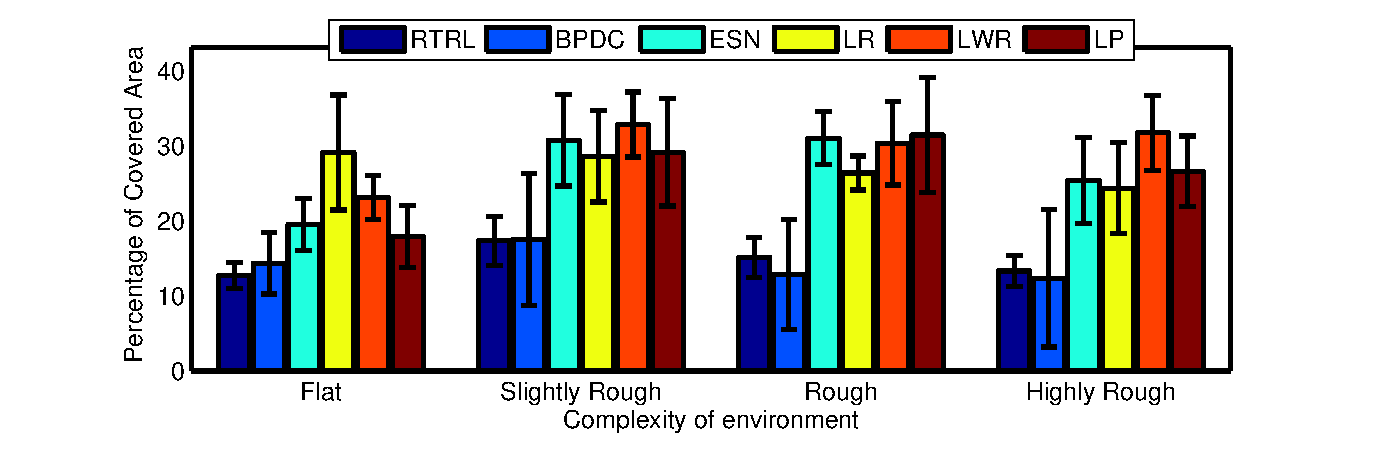
\includegraphics[scale=0.65]{Area_Env.eps}
\centering
\caption{Performance of all the internal models in terms of area coverage }
\label{fig:Area_Env}
\end{figure}


\subsection*{The environments' complexity affects the complexity of generated behaviours.}

Although that an indication of a dependency between the environment and behaviours' complexity was shown in figure \ref{fig:Area_Env}, this relationship is illustrated more clear in figure \ref{fig:Area_sortEnv} where the evolution of area coverage is plotted over the different environments which are sorted in order of ascending complexity.     

\begin{figure}[H]
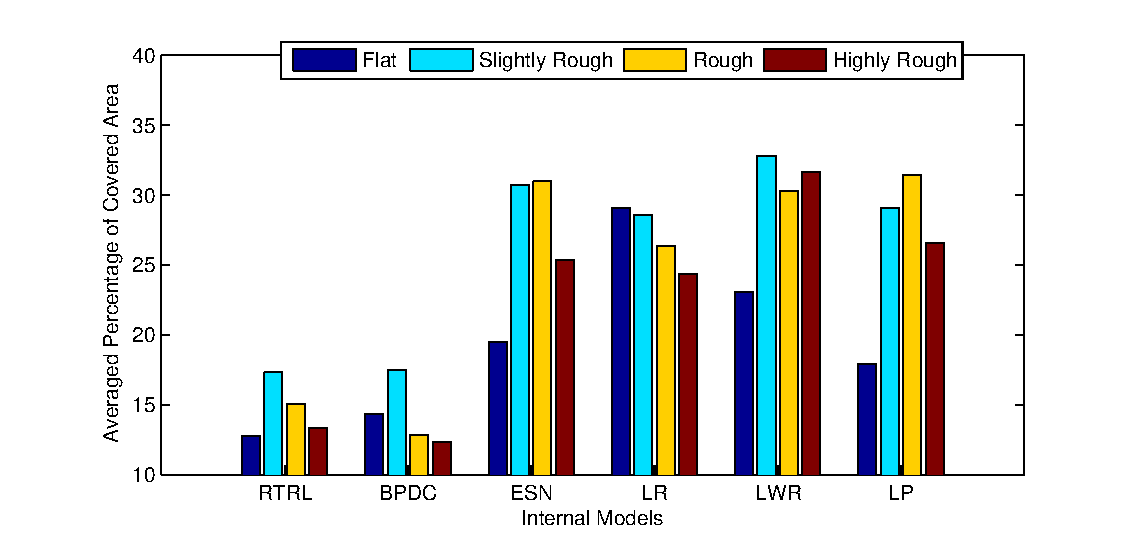
\includegraphics[scale=0.8]{Area_sortEnv.eps}
\centering
\caption{Covered area by each model sorted by environments complexity  }
\label{fig:Area_sortEnv}
\end{figure}

Based on this plot it is clear that all models perform better in the slightly rough environment compared to the flat environment except from the LR which has similar performance in both environments but a large variation in the flat environment. In the rough environment, two models increased their performance (LP, ESN) but at the other hand the performance of LWR and RTRL had a slight decrease but their performance was not worse than the flat environment. The BPDC and LR exhibit a decreasing performance as the environments' complexity increases. Finally in the most complex environment, the LWR has increased its performance contrary to all the other models.   

It is clear that the environment has an impact on the internal models, this impact depends on the type of the model. Thus, most models (RTRL, BPDC, ESN and LP) perform better in environments of medium complexity contrary to the LR which requires a low complex environment and LWR which has a steady performance in the more complex environments. Thus was observed that an explorative behaviour is likely to occur in more complex environments than the simpler ones. The reduce of the models' performance in the highly rough environment can be explained by the fact that the robot has to generate a "climbing" behaviour for exploring its environment. This behaviour can be considered more complex than the combination of steering and forward heading that are required for exploring simple environments.

Summarizing, it is safe to say that there are significant outcomes which support the hypothesis that more complex environments cause the emergence of complex behaviours. Also there are indications that the models' attributes, such as predictability and complexity affect the behaviour. The impact of those attributes are examined with detail in the rest of this section.    

\subsection*{The quality of the model affects the generated behaviours}

Figure \ref{fig:Area_Error} is a scatter plot of the covered area and MSE for all the internal models and environments. The general outcome is that there are three clusters that exhibit a different behaviour. One that has large MSE and small area coverage and is formed by the BPDC, the other has low MSE and low area coverage and includes the results obtained by the RTRL and also the results obtained by applying the LP and the ESN in the flat environment. The last cluster consist of the results obtained by applying LP and ESN in the more complex environments and by applying LR and LWR in all the environments.

Should be denoted here that the low area coverage of ESN and LP in the flat environment is a result of the environments' complexity and not of the MSE since the MSE is not significantly larger in this compared to the other environments. Thus, for the evaluation of this hypothesis, is safe to ignore the values obtained by ESN and LP in the flat environment.

The covered area depends on the MSE when the errors are bigger than $0.01$, as it derives comparing the covered area when the robot uses the models BPDC and LR against the models ESN, LP and LWR. The low performance of RTRL, despite the low error is an indication that the area coverage does not depend only on the MSE but also on the models' structure.  


\begin{figure}[H]
\includegraphics[scale=0.8]{Area_Error.eps}
\centering
\caption{Dependence between MSE and area coverage }
\label{fig:Area_Error}
\end{figure}

Thus looking at the models that have similar structure, LP-LR and ESN-BPDC, it is clear that the MSE has an impact on the achieved area coverage. Therefore, the hypothesis that the predictability of the models' affects the emergence of behaviours is partially valid because it was proved that the models' structure also affects the behaviours. So can be concluded that if the predictability of the models is decent then the emergence of behaviours mainly depends on their structure. This dependence will be further investigated.  

\subsection*{Complex models result to complex behaviour }

From the previous analysis arises the fact that there should be a dependency between models' complexity and generated behaviours. For evaluating this hypothesis, the models should be classified according to their complexity. Although that there are methods for measuring the complexity, in this approach, we are more interested about the structure of the models such as the number of models' elements and their interactions than the assumptions that each model makes about the form of the inputs-outputs mapping or the computational complexity of the learning rule.

For those reasons, the classification of models' according to their complexity was made based on a naive approach. The factors that are taken into account sorted in order of significance are: the number of structural elements, the number of interactions between those elements, the assumptions made about the form of inputs-outputs mapping and the last and less significant factor is the computational complexity of the learning rule.   

Figure \ref{fig:Area_Compl} illustrates the models sorted in order of ascending complexity as result of the described approach. Based on the first criterion, the regression methods are less complex than the RNNs since they have less interacting elements. In the class of regression methods all models have the same number of interacting elements and interactions between them, thus according to the third criterion the LR is the less complex method since it assumes a linear input-output mapping contrary to the other two which are not making any assumption. Finally, the LWR is classified as the most complex algorithm because the learning rule is more complex than the learning rule of LP.
Following the same procedure at the RNNs, the RTRL was classified as the most simple because the RNN consists of less nodes. Between BPDC and ESN, which have the same structure, the most complex is ESN because of its learning rule.  
 
\begin{figure}[H]
\includegraphics[scale=0.94]{Area_Complex.eps}
\centering
\caption{Dependence between models' complexity and area coverage}
\label{fig:Area_Compl}
\end{figure}

Thus a general outcome from figure \ref{fig:Area_Compl} is that using the regression methods, a better area coverage is achieved compared to more complex RNNs. An interesting observation is that RTRL and BPDC have similar performance despite the large difference in their predictability. This can be explained by the fact that BPDC uses a reservoir of fixed weights which makes the model more sensitive to the changes of inputs. Recalling that, for minimizing the time loop error (section \ref{sec:tle}) the model has to be sensitive to inputs' changes, it is safe to say that the use of a reservoir in RNNs increases the models sensitivity. This outcome is further supported by comparing the area coverage between RTRL and ESN which have similar predictability but more complex behaviour emerges by using ESN.  

Also given that, the general performance of regression methods is better than the performance of ESN, can be concluded that a large number of structural elements with many interactions result to a less sensitive model which does not drive the robot to the emergence of complex behaviours. Thus, the initial hypothesis that more complex models result to more complex behaviours is not valid. It is proved that an opposing relation exists, less complex models result to more complex behaviours because the models' sensitivity is larger when it consists of few structural elements. 

\subsection*{Dependence between models' predictability and environment complexity}

For investigating if the complex models have a better predictability in complex environments, the models are again sorted according to their complexity following the same procedure that described later in the section. Figure \ref{fig:Error_Compl} illustrates the averaged MSE of every model over the different environments. The BPDC has the highest error as result of the poor performance of its learning rule which takes into account the error of the last two consecutive time steps for updating the weights. Observing the other models, the error of the least complex model(LR)is the highest while there is not any significant difference between the predictability of the more complex models.

A point that should be highlighted is that, at the majority of models, the errors in the flat environments are slightly bigger than the the errors in the other environments. This can be explained when the robots hits the wall. In this occasion, that happens frequently in the flat environment, the relation between between motor commands (inputs) and sensory values (outputs) has a significant and instant change that makes the models incapable to learn because.   

\begin{figure}[H]
\includegraphics[scale=0.78]{Error_Complex.eps}
\centering
\caption{Dependence between models' complexity and predictability }
\label{fig:Error_Compl}
\end{figure}

Summarizing, can be concluded that the mapping between inputs and outputs is relatively simple and does not significantly changes in different environments. Thus there is not the need of using a complex model in complex environments. Based on those outcomes the hypothesis that models' predictability is affected by the environments' complexity is not valid.  
\include{Evaluation}

\chapter{Conclusion and Discussion}
\label{ch::cd}
In this thesis was presented a study of the internal models' impact on a robot which controlled by an homeokinetic controller. The control scheme is based on the process of self-organization that occurs in nature and describes the evolution of several physical, chemical and social phenomena. Through self-organization, the agents of a system that are initially in unordered state can exhibit an order that arises from environmental stimuli which also affect the emergence of the system's patterns. Those patterns do not depend on a single agent but is a result of the system's interaction with the environment. Thus, the application of this process in robotics control requires a module that will make the robot capable to maintain a belief about its interaction with the environment for reacting according to environmental changes.        
The belief about the robot's environment is encoded in the internal model. Through this, the robot can predict the effect of its actions to the environment.    

In the applied control scheme the robot is considered to be the whole system and its motors are the agents of this system. In which is applied the principle of homeokinesis. Through homeokinesis is achieved an organization at the motor commands, which is not externally controlled (there is not an externally defined goal) but depends on internal factors such as the robot's interaction with the environment and its ability to predict its future state. This is achieved by exploiting the dynamics of neurons in a closed sensorimotor loop which exhibits properties that are similar to the occurrence of self-organization in nature. The robot's agents change state in order to minimize the time loop error which depends on the robot's internal model.

It is clear from the mathematical formulation of the Time Loop Error that internal models has a significant role in the change of motor commands. Particularly, both models' predictability and sensitivity are significant. This fact makes important the study of different predictors' types, thus in this thesis were examined both recurrent neural networks and regression techniques. The class of recurrent neural networks includes internal models of different structure and learning rules. Namely was applied a fully connected recurrent neural network trained with the real time recurrent learning rule and two reservoir recurrent networks using back-propagation decorrelation and delta training rule. The tested repossession methods are the linear regression, the non-parametric method of locally weighted regression and a linear predictor in which was used the delta rule for weights' adaptation contrary to the other two where were used the least square estimator for the derivation of the weights'.

Those models were applied in the homeokinetic control scheme for evaluating four main hypotheses. Particularly, were investigated the impact of the models predictability and complexity to the emergence of behaviours, the dependency between environments' complexity and behavioural complexity and the effect of complex environments on the models' predictability.The evaluation of those hypotheses was based on the results of multiple simulations for each one of the internal models in four environments of different complexity. The results denote that more complex behaviours emerge in complex environments. Also the robot's behaviour does not heavily depend on the models' predictability but on models' complexity. Because, it was observed that, between models which had similar predictability, more complex behaviours emerged by using less complex models. Finally, was concluded that models are capable of predicting the feature sensory values regardless the complexity of the environment. 
\section*{Criticism}  
Despite that the results provide a reliable base for evaluating the hypotheses, the tunable parameters of internal models (number of nodes, learning rate, etc.) were set arbitrarily. Since they affect the performance of the predictors, it should exist a process for adjusting them in order to minimize the regularization error. Such processes involve the collection of inputs and their corresponding outputs at each time step, then this dataset is partitioned in a training and an evaluation set. Different combinations of the tunable parameters are applied in the training test and are tested in the evaluation set. The parameters that are minimizing the evaluation error are selected. Using this process, is ensured the best possible predictability of each model.

Another issue that should be highlighted is that      


\include{}

% \include{chap2}
%% ... etc ...

%%%%%%%%
%% Any appendices should go here. The appendix files should look just like the
%% chapter files.
%\appendix
%\include{appendix1}
%% ... etc...

%% Choose your favourite bibliography style here.
\bibliographystyle{apalike}

%% If you want the bibliography single-spaced (which is allowed), uncomment
%% the next line.
 %\singlespace

%% Specify the bibliography file. Default is thesis.bib.
\bibliography{thesis}

%% ... that's all, folks!
\end{document}
